\documentclass[letterpaper]{article}
\usepackage{aaai}
\usepackage{times}
\usepackage{helvet}
\usepackage{courier}
\setlength{\pdfpagewidth}{8.5in}
\setlength{\pdfpageheight}{11in}
%
\usepackage{amsfonts}

%
\usepackage{mathrsfs}
\usepackage{amsthm,amsmath,amsfonts,amssymb}

\usepackage{bm}
\usepackage[mathscr]{eucal}
\usepackage{stmaryrd}
\usepackage{paralist}
\usepackage{indentfirst}
\usepackage{graphicx}
\setkeys{Gin}{width=0.2\textwidth,height=35mm}
\usepackage{subfigure}
% for algorithm
\usepackage[ruled]{algorithm}
\usepackage{algpseudocode}

% hyperref
\usepackage[colorlinks,linkcolor=blue, filecolor=blue,urlcolor=blue,citecolor=blue]{hyperref}
\usepackage{url}
\newcommand{\Sca}[3]{{#1}^{(#2)}_{i_#2#3}}%Scalar with superscript and subscript
\newcommand{\Scah}[3]{h^{(#1,#2)}_{#3}(\V{x}_{i_#1})}

%% -------
%% Tensor
%% -------
\newcommand{\T}[1]{\boldsymbol{\mathscr{\MakeUppercase{#1}}}}

\newcommand{\KT}[1]{\left\llbracket #1 \right\rrbracket}

%% -------
%% Vector
%% -------
\newcommand{\V}[1]{{\bm{{\MakeLowercase{#1}}}}}
% Vector with superscript and subscript
\newcommand{\VnC}[3]{\V{#1}^{(#2)}_{#3}}
% norm one of r-th cloumn
\newcommand{\Nrocl}[2]{\norm{\VnC{a}{#1}{*#2}}{1}}

\newcommand{\Varow}[1]{\V{a}^{(#1)}_{i_#1*}}
\newcommand{\Vacol}[1]{\V{a}^{(#1)}_{*r}}

%% -------
%% Matrix
%% -------
\newcommand{\M}[1]{{\bm{\mathbf{\MakeUppercase{#1}}}}}
%Matrix with superscript
\newcommand{\Mn}[2]{\M{#1}^{(#2)}}

% p-norm
\newcommand{\norm}[2]{\|#1\|_{#2}}

%% ------------
%% reference
%% ------------

% reference:definition
\newcommand{\Def}[1] {\hyperref[def:#1] {Definition~\ref*{def:#1}}}
% reference:equation
\newcommand{\Eqn}[1] {\hyperref[eq:#1]  {Equation~\ref*{eq:#1}}}
% reference:figure
\newcommand{\Fig}[1] {\hyperref[fig:#1] {Figure~\ref*{fig:#1}}} %
% reference:table
\newcommand{\Table}[1] {\hyperref[table:#1] {Table~\ref*{table:#1}}} %
% reference:lemma
\newcommand{\Lem}[1] {\hyperref[lem:#1] {Lemma~\ref*{lem:#1}}} %
% reference:theorem
\newcommand{\Theo}[1]{\hyperref[lem:#1] {Theorem~\ref*{theo:#1}}} %
% reference:property
\newcommand{\Prop}[1]{\hyperref[prop:#1]{Property~\ref*{prop:#1}}} %
% reference:algorithm
\newcommand{\Alg}[1] {\hyperref[alg:#1] {Algorithm~\ref*{alg:#1}}}
\newcommand{\AlgLine}[2]{\hyperref[alg:#1]{line~\ref*{line:#2} of Algorithm~\ref*{alg:#1}}}
\newcommand{\AlgLines}[3]{\hyperref[alg:#1]{lines~\ref*{line:#2}--\ref*{line:#3} of Algorithm~\ref*{alg:#1}}}

\newcommand{\Coord}{(i_1,i_2,\ldots,i_N)}



\newtheorem{definition}{Definition}
\newtheorem{lemma}{Lemma}
\newtheorem{theorem}{Theorem}


\begin{document}
\title{Central Sampling for Top t Retial Processing}
\date{}
\author{}
\maketitle

\section{Introduction}

In fashion recommendation system, it is an essential task to find the most relevant items given a specific user. Similar application can also be found in information retrieval. If we consider all users as a set of feature vectors, and items are also represented by vectors with the same dimension. Then this problem can be abstracted to matrix multiplication tasks when we define the relevance as the inner product of two vectors, which known as maximum inner-product search(MIPS). An application of MIPS is the  matrix-factorization framework in recommender system\cite{KoYe09}. However, we may have more than one categories of items, that is, we have more than one item matrices and relevance of user to a suit of items may defined by another way. And the tensor factorization models was used for multi-items recommendation\cite{Rendle10} and outfit recommendation\cite{HuYiLa15}. Those problem can be summarized into the top-t problem:

\begin{definition}\label{def:DefinitionTopt}
(top-t Retrial.) Suppose $S_1,S_2,..S_N$ are set for $N$ different kind of items(tags). $\V{t}_{i_1},\V{t}_{i_2},...,\V{t}_{i_N}$ are items in each set that are all represented by same dimension vector. And there is a ranking function $f(\V{t}_{i_1},\V{t}_{i_2},...,\V{t}_{i_N})$: find the $t$ tuples $(i_1,i_2,...,i_N)$ that have the largest or lowest ranking function value of all.
\end{definition}

For two sets case, there are three ranking functions that used widely, Euclidean distance, cosine similarity and inner-product. And when we fix one of item, say ${i_1}$, this is the query retrial problem.
\subsection{Notations}

The item matrix that consists of a mount of feature vectors with the same dimension is represented as $\M{A} =
[\V{a}_{1},\V{a}_{2},\cdots,\V{a}_{R}]\in R^{L\times R}$.  Without loss of generality, we use $R$ to represent the dimension of a feature vector, and $L$ as the number of items in one category. In one category situation, when we evaluate the relevance of an item to a user by the inner-product which is $\M{A}(i,:)\V{u}=(a_{i1},a_{i2},\ldots,a_{iR})\cdot\V{u}$, it equals to find the max value in $\V{q} = \M{a}\V{u}$.

To be more general, we consider a set of matrices $\M{A}^{(n)},n = 1,...,N$ consisting of item vectors, and the ranking function $x_\V{i} = \sum_{r=1}^{R}\Sca{a}{1}{r}\cdot\Sca{a}{2}{r}\cdots\Sca{a}{N}{r}$, which degenerate into inner-product when $N=2$. By this definition, the recommendation for one user is an exceptional case when we consider one of matrix as a single vector. For convenience, we call $\V{i} = (i_1,i_2,\ldots,i_N)$ the coordinate or multi-index. The hypothesis of relevance criterion is reasonable and used widely in recommendation system for multi-category. If we rearrange the actual values as a $N$-way tensor, these items matrices would be the CP decomposition of this tensor.


We use the some definition vector and matrix norm refereed in \cite{BaPiKoSe15}. Suppose $\V{v}\in R^n$ is a vector and $\M{M}\in R^{m\times n}$ is a matrix. The norm $\norm{*}{1}$ operation is defined as followed:
\[
    \norm{\V{v}}{1} = \sum_{i=1}^{n}|v_i|
    \ \  and \ \
    \norm{\M{M}}{1} = \sum_{i=1}^{m}\sum_{j=1}^{n}|m_{ij}|
\]

We also use different letters to represent the tensor, matrix, etc. And some frequently used notations are listed in ~\Table{Notation}.

\subsection{Tensor decomposition}

Consider a $N$-order tensor, $\T{X}$ with size $L_1\times L_2\times\ldots\times L_N$, the CP decomposition\cite{KoBa09} of this tensor is

\begin{equation}\label{eq:CPDecomposition}
\T{X}= \KT{ \Mn{A}{1},\dots,\Mn{A}{N}} =
\sum_{r=1}^{R}\VnC{A}{1}{r} \circ \cdots \circ \VnC{A}{N}{r}
\end{equation}

where

\begin{gather*}\label{eq:ColumnVectorsForm}
\M{A}^{(1)} =
\begin{bmatrix}\VnC{a}{1}{1},\VnC{a}{1}{2},\cdots,\VnC{a}{1}{r}\end{bmatrix}\in R^{L_1\times R}\\
\M{A}^{(2)} =
\begin{bmatrix}\VnC{a}{2}{1},\VnC{a}{2}{2},\cdots,\VnC{a}{2}{r}\end{bmatrix}\in R^{L_2\times R}\\
\vdots\\
\M{A}^{(N)} =
\begin{bmatrix}\VnC{a}{N}{1},\VnC{a}{N}{2},\cdots,\VnC{a}{1}{r}\end{bmatrix}\in R^{L_N\times R}\\
\end{gather*}

In ~\Eqn{CPDecomposition}, $\M{A}^{(n)}$ is the factor matrix, and the column size $R$ represents the rank of this tenors, which is also the dimension of feature vector. The vector $\VnC{a}{n}{r}$ is the $r$-th column of matrix $\Mn{A}{n}$.

The element in $\T{X}$ satisfies the following equation:

\begin{equation}\label{eq:ValueInTensor}
x_\V{i} = \sum_{r=1}^{R}\Sca{a}{1}{r}\cdot\Sca{a}{2}{r}\cdots\Sca{a}{N}{r}
\end{equation}

The indexes vector $\V{i}$ is a shorthand for multi-index $(i_1,i_2,\ldots,i_N)$. And the value in tensor is what we need to find when we have those factor matrices. It is a time-consuming task to compute all value of each element. In following sections, we will introduce the diamond sampling\cite{BaPiKoSe15} for approximating matrix multiplication tasks which is an improvement of wedge sampling\cite{Cohen97}. Then we extend this method to handle the tensor factorization models.

\begin{table}[t]
  \label{table:Notation}
  \centering
  \begin{tabular}{|c|c|}
    \hline
    Notations & Explanation \\
    \hline
    $\T{A}$ & tensor \\
    $\M{A}$ & matrix \\
    $\Mn{A}{n}$ & $n$-th factor matrix of tensor\\
    $\V{A}_{*r},\V{A}_r$ & $k$-th column of matrix \\
    $\V{A}_{i*}$ & $i$-th row of matrix \\
    $\V{A}$ & vector \\
    $a_{ir}$ & element of matrix, a scalar\\
    \hline
  \end{tabular}
  \caption{Notation}
\end{table}



\section{Related work}

There are many splendid work on finding the max dot-product of two sets of vectors called MAD search\cite{BaPiKoSe15} and MIPS(Maximum Inner Product Search)\cite{Cohen97,Ram12}. We analysis those similar work based on the probabilistic method, which can be called sampling. The main idea of those method is to sample the indexes or coordinate $\V{i}$ that is proportional to the value of this coordinate $x_{\V{i}}$. The most representative work are diamond sampling and wedge sampling. In following section we will exten the diamond sampling method to deal with $N$ factor matrices.


\section{Diamond Sampling Algorithm}

The diamond sampling is a way to sample the index-pair $(i,j)$ proportional to $c^2_{i,j}$ in matrix multiplication $\M{C} = \M{A}\M{B}^T$. This method consider a matrix $A$ with size $m\times n$ as a weighted bipartite graph $G_{A}$. Meanwhile, in the adjacent matrix of this graph, using $0$(instead of $\infty$) to represent the two vertices are not adjacent. And the adjacent matrix of $G_{A}$ is:
\[
\left(
  \begin{array}{cc}
    \V{0}_{m\times m} & A \\
    A^T & \V{0}_{n\times n} \\
  \end{array}
\right)
\]

\subsection{Sampling via Graph representation}

In equation \ref{eq:CPDecomposition}, we have $N$ factor matrices $\Mn{A}{1},\dots,\Mn{A}{N}$.
Those $N$ factor matrices can be represented by a weighted $(N+1)$-partite graph $G_{T}$. And we call those $N+1$ partitions as partition $\overline{V},V_{1},V_{2},\ldots,V_{N}$, in which partition $V_{n}$ has $L_n$ vertexes and partition $\overline{V}$ has $R$ vertexes. We call $v^n_{i_n}$ the $i_n$-th vertex in partition $V_{n}$, and $\overline{v}_{r}$ the $r$-th vertex in partition $\overline{V}$. Every two vertexes from different partition classes $V_i,V_j,i,j\in {1,2,\ldots,N}$ are not adjacent. A vertex $\overline{v}_r$ in $\overline{V}$ is only adjacent to vertexes $v^n_i$ in $V_n$ when $\Sca{a}{n}{r}$ is non-zero and the edge weight $\Sca{a}{n}{r}$. And the adjacent matrix of $G_{T}$ is :
\[
\left(
  \begin{array}{cccc}
    \M{0}_{R\times R}   & {\Mn{A}{1}}^T         & \ldots & {\Mn{A}{N}}^T \\
    \Mn{A}{1}           & \M{0}_{L_1\times L_1} & \ldots & \M{0}_{L_1\times L_N} \\
    \vdots              & \vdots                & \ddots & \vdots \\
    \Mn{A}{N}           & \M{0}_{L_N\times L_1} & \ldots & \M{0}_{L_1\times L_N} \\
  \end{array}
\right)
\]

Under the graph presentation, we define an event $\varepsilon_{\V{i},r',r}$  consisting of three phases:
\begin{itemize}
  \item phase 1. Pick an edge $e=(v^1_{i_1},\overline{v}_r)$;
  \item phase 2. Walk $N-1$ times from the $\overline{v}_r$ to other partitions $V_2,\ldots,V_N$, arrive at $v^2_{i_2},v^3_{i_3},\ldots,v^N_{i_N}$;
  \item phase 3. Walk from $v^1_{i_1}$ to $\overline{V}$ and end in $\overline{v}_r'$.
\end{itemize}

When the event $\varepsilon_{\V{i},r',r}$ happened, we give a score according to indexes $\V{i}:(i_1,i_2,\ldots,i_N)$. We will assign each phase probabilities so that the final score of $\V{i}:(i_1,i_2,\ldots,i_N)$ will be a good estimation of $x_{\V{i}}$.

The sampling algorithm is shown in ~\Alg{DiamondSampling}.

\begin{algorithm}[t]
    \caption{Diamond Sampling with factor matrixes}
    \label{alg:DiamondSampling}
    Given factor matrix $\M{A}^{(n)}\in R^{L_n\times R}, n = 1,2,\ldots,N$.\\
    Let $s$ be the number of samples.
    \begin{algorithmic}[1]
    \For{all $(i_1,r)$}
    \State $w_{i_1r} \leftarrow \mid \Sca{a}{1}{r}\mid
    \norm{\Varow{1}}{1}\norm{\Vacol{2}}{1}\ldots\norm{\Vacol{N}}{1} $
    \EndFor
    \State Initialize an empty map for coordinate.
    \For{$ \ell = 1,\ldots,s$}
    \State Sample $(i_1,r)$ with probability $w_{i_1r}/\norm{\V{W}}{1}$        \label{line:phase1}
    \For {$n=2,...,N$}
    \State Sample $i_n$ with probability $|\Sca{a}{n}{r}|/\norm{\Vacol{n}}{1}$
    \label{line:phase2}
    \EndFor
    \State Sample $r'$ with probability $|\Sca{a}{1}{r'}|/\norm{\Varow{1}}{1}$
    \label{line:phase3}
    \State \label{line:scoring}
        Get score: $sgn(\Sca{a}{1}{r}\cdots\Sca{a}{N}{r}\cdot\Sca{a}{1}{r'})
    \Sca{a}{2}{r'}\cdots\Sca{a}{N}{r'}$
    \If {the map has key $i_1,i_2,\cdots,i_N$}
    \State  Set a new key with this score
    \Else
    \State Increase the key by this score
    \EndIf
    \EndFor
    \end{algorithmic}
\end{algorithm}

\subsection{Probability in Each Phase}

In this part, we introduce the probabilities in each phase of event $\varepsilon_{\V{i},r',r}$.

\begin{itemize}
  \item Walking with probability  (~\AlgLines{DiamondSampling}{phase2}{phase3})

  In phase 2 we start from a vertex in $\overline{V}$ to $V_i$, and phase 3 from a vertex in $V_1$ to $\overline{V}$. We choose the path(edge) according to its weight. That is in phase 3, picking $r\in\{1,2,\ldots,R\}$ with probability $|\Sca{a}{1}{r'}|/\norm{\Varow{1}}{1}$ or given $r$, in phase 2, picking $i_n\in\{1,2,\ldots,L_n\}$ with probability $|\Sca{a}{n}{r}|/\norm{\Vacol{n}}{1}$.

  \item Picking an edge (~\AlgLine{DiamondSampling}{phase1})

  When we pick an edge $e=(v^1_{i_1},\overline{v}_r)$ in phase 1, we are picking the vertexes pair $(v^1_{i_1},\overline{v}_r)$. Beforehand, we assign each pair a probability when $ \Sca{a}{1}{k} \neq 0 $:
  \[
    p(i_1,r) = |\Sca{a}{1}{r}|\norm{\Varow{1}}{1} \norm{\Vacol{2}}{1} \ldots \norm{\Vacol{N}}{1} / \norm{\V{W}}{1}
  \]
  Where
  \[
    \norm{\V{W}}{1} = \sum_{i_1,r}\mid \Sca{a}{1}{k}\mid \norm{\Varow{1}}{1} \norm{\Vacol{2}}{1} \ldots \norm{\Vacol{N}}{1}
  \]
  Then we pick the pair $(v^1_{i_1},\overline{v}_r)$ according the probability $p(i_1,r)$.
\end{itemize}

\subsection{Scoring Sampled Coordinates}

Totally, we do $s$ times sampling, and each sample we will get an coordinate $\V{i} = (i_1,i_2,\ldots,\i_N) $. If this coordinate has not been sampled previously, let the score of this coordiante in the $\ell $-th turn be
\[
\M{X}_{\V{i},\ell}  = sgn(\Sca{a}{1}{r}\cdot\Sca{a}{2}{r}\cdots\Sca{a}{N}{r}\cdot\Sca{a}{1}{r'}) \Sca{a}{2}{r'}\cdots\Sca{a}{N}{r'},
\]
and make $\widehat{x}_{\V{i}} = \M{X}_{\V{i},\ell}$ into a set where we save the scores. Otherwise, increase $\widehat{x}_{\V{i}}$ in the set by $\M{X}_{\V{i},\ell}$. It is shown in ~\AlgLine{DiamondSampling}{scoring}. For $\V{i}$ that not be sampled in $\ell$-th turn, we can assume that $\M{X}_{\V{i},\ell}=0$. So
\[
\widehat{x}_{\V{i}} = \sum_{\ell} \M{X}_{\V{i},\ell}
\]

In the next part, we will show that $\widehat{x}_{\V{i}}$ is a good estimation of $x_{\V{i}}^2$.

\subsection{Extracting Top-$t$ Largest Value}

We use the sampling score $\widehat{x}_{\V{i}}$ and coordinate set $\V{i}$ to find the top-t largest value in $\T{X}$ when given $N$ factor matrices. Let $\Omega_s = \{\V{i}_j|j = 1,2,\ldots,s\}$ be the coordinates have been sampled.

To reduce the computing, a pre-sort is carried out. It sort the scores $\widehat{x}_{\V{i}}$ and reserve the top-$t'$ elements. Obviously, $t'$,which called budget, is always much larger than $t$.

Then we compute the actual value $x_{\V{i}}$ of the coordinates in the less small set $\Omega_{t'} = \{\V{i}|\widehat{x}_{\V{i}}\geq \widehat{x}_{\V{i'}},\forall i'\in \Omega_{s} \backslash \Omega_{t'}\}$. And the top-$t$ largest value's coordinates will be $\Omega_{t}=\{\V{i}|x_{\V{i}}\geq x_{\V{i'}},\forall i' \in \Omega_{t'} \backslash \Omega_{t} \}$.

The reason to do so is that although the score $\widehat{x}$ is a good estimation, the variance is much higher in practical. And the budget $t'$ is a tradeoff between accuracy and computation. The algorithm for finding the top-$t$ largest value is shown in ~\Alg{Topt}.
\begin{algorithm}[t]
    \caption{Finding top-$t$ largest value}
    \label{alg:Topt}
    Given factor matrix $\M{A}^{(n)}\in R^{L_n\times R}, n = 1,2,\ldots,N$.\\
    Let $s$ be the number of samples, $t'$ be the budget.
    \begin{algorithmic}[1]
    \State Sample the score $\widehat{x}_\V{i}$ using ~\Alg{DiamondSampling} and record the coordinates set $\Omega_s$ have been sampled.
    \State Sort the score to extract
    \[
        \Omega_{t'} = \{\V{i}|\widehat{x}_{\V{i}}\geq \widehat{x}_{\V{i'}},\forall i'\in \Omega_{s} \backslash \Omega_{t'}\}
    \]
    \State Compute the actual value $x_{\V{i}}$ of each coordinate in $\Omega_{t'}$
    \State Sort the actual value to extract
    \[
        \Omega_{t}=\{\V{i}|x_{\V{i}}\geq x_{\V{i'}},\forall i' \in \Omega_{t'} \backslash \Omega_{t} \}
    \]
    \end{algorithmic}
\end{algorithm}

\subsection{Correctness and Error Bounds}

As we defined previously, the event $\varepsilon_{\V{i},r',r}$ is picking a pair $(v^1_{i_1},\overline{v}_r)$ then pick paths from $V_1$ to $\overline{V}$ and some addition pathes from $\overline{V}$ to $V_i,i\in{2,\ldots,N}$. And we assume that $\M{X}_{\V{i},\ell},\ell\in\{1,2\ldots,s\}$ are independent. Under these assumptions, we give two lemmas.

\begin{lemma}\label{lem:Expectation}
The expectation of $\widehat{x}_{\V{i}}$ equals to $sx^2_{\V{i}}/\norm{\M{W}}{1}$.
\end{lemma}


\begin{proof}[Proof:]
The final score $\widehat{x}_{\V{i}} = \sum_{\ell=1}\M{X}_{\V{i},\ell}$. And
\begin{equation}\label{eq:Expectation}
\mathbb{E}[\widehat{x}_{\V{i}}] = \sum_{\ell=1}\mathbb{E}[\M{X}_{\V{i},\ell}]=s\mathbb{E}[\M{X}_{\V{i},1}]
\end{equation}

The probability of $\varepsilon_{\V{i},r',r}$ is

\begin{align*}
Pr(\varepsilon_{\V{i},r',r})
%& = Pr( {\rm pick\ } (v^1_{i_1},\overline{v}_r))
%Pr( {\rm walk\ to\ } \overline{v}_r' | {\rm given\ }v^1_{i_1} )
%Pr( {\rm walk\ to\ } v^2_{i_2} | {\rm given\ }\overline{v}_r) \cdots Pr( {\rm walk\ to\ } v^N_{i_N} | {\rm given\ }\overline{v}_r ) \\
& = Pr({\rm phase\ 1})Pr({\rm phase\ 2})Pr({\rm phase\ 3})\\
&=\frac{w_{i_1r}}{\norm{\V{W}}{1}}
  \frac{|\Sca{a}{2}{r}|}{\norm{{\VnC{a}{2}{*r}}}{1}}\cdots
  \frac{|\Sca{a}{N}{r}|}{\norm{{\VnC{a}{N}{*r}}}{1}}
  \frac{|\Sca{a}{1}{r'}|}{\norm{{\VnC{a}{1}{i_1*}}}{1}}\\
%&=\frac{    |\Sca{a}{1}{r}|\norm{{\VnC{a}{1}{i_1*}}}{1}\norm{{\VnC{a}{2}{*r}}}{1}\cdots\norm{{\VnC{a}{N}{*r}}}{1}   }{  \norm{\V{W}}{1}  }\frac{|\Sca{a}{1}{r'}|}{\norm{{\VnC{a}{1}{i_1*}}}{1}} \frac{|\Sca{a}{2}{r}|}{\norm{{\VnC{a}{2}{*r}}}{1}}\frac{|\Sca{a}{N}{r}|}{\norm{{\VnC{a}{N}{*r}}}{1}}\\
&=\frac{    |\Sca{a}{1}{r'}\Sca{a}{1}{r}\cdots\Sca{a}{N}{r}|    }{\norm{\V{W}}{1}}
\end{align*}

Then we get the probability of one walk:

\begin{equation}\label{eq:ProbabilityOneWalk}
Pr(\varepsilon_{\V{i},r',r})=\frac{|\Sca{a}{1}{r'}\Sca{a}{1}{r}\cdots\Sca{a}{N}{r}|}{\norm{\V{W}}{1}}
\end{equation}

Using \Eqn{Expectation} and \Eqn{ProbabilityOneWalk}. The expectation
\begin{align*}
&\mathbb{E}[x_{\V{i}}/s] = \mathbb{E}[\M{X}_{\V{i},1}]\\
&=\sum_{r,r'} Pr(\varepsilon_{\V{i},r',r}) sgn(\Sca{a}{1}{r'}\Sca{a}{1}{r}\cdots\Sca{a}{N}{r})
\Sca{a}{2}{r'}\cdots\Sca{a}{N}{r'}\\
%&=\frac{\sum_{r,r'}|\Sca{a}{1}{r'}\Sca{a}{1}{r}\cdots\Sca{a}{N}{r}|sgn(\Sca{a}{1}{r'}\Sca{a}{1}{r}\cdots\Sca{a}{N}{r})
%\Sca{a}{2}{r'}\cdots\Sca{a}{N}{r'}}{\norm{\M{W}}{1}}\\
&=\frac{\sum_{r,r'} \Sca{a}{1}{r}\cdots\Sca{a}{N}{r}\Sca{a}{1}{r'}\cdots\Sca{a}{N}{r'}}{\norm{\V{W}}{1}}\\
&=\frac{(\sum_{r}\Sca{a}{1}{r}\Sca{a}{2}{r}\cdots\Sca{a}{N}{r})^2}{\norm{\V{W}}{1}}\\
&=\frac{x_{\V{i}}^2}{\norm{\V{W}}{1}}
\end{align*}
\end{proof}



\begin{lemma}\label{lem:Bound}
Fix $\varepsilon > 0$ and error probability $\sigma \in (0,1)$. Assuming all entries in factor matrices are nonnegative and at most $K$. If the number of samples
\[
s \leq 3K^{N-1}\norm{\V{W}}{1}\log{(2/\sigma)}/(\varepsilon ^2{x_{\V{i}}}^2),
\]
then
\[
Pr[|{\widehat{x}_{\V{i}}}\norm{\V{W}}{1}/s-{x_{\V{i}}}^2| \geq \varepsilon{x_{\V{i}}}^2] \leq \sigma
\]
\end{lemma}

\begin{proof}[Proof:]
Let
\[
    y_{\V{i}} = \sum_{\ell}\M{Y}_{\V{i},\ell} = \sum_{\ell}\M{X}_{\V{i},\ell}/K^{N-1}
\]
Where $\M{Y}_{\V{i},\ell}$ is in $[0,1]$ for $\M{X}_{\V{i},\ell}$ is in $[0,K^{N-1}]$ and $y_{\V{i}}$ is a sum of random variables in $[0,1]$.
Applying the Chernoff bound,
\[
Pr[y_{\V{i}} \geq \mathbb{E}[y_{\V{i}}]] < \exp{(-\epsilon^2\mathbb{E}[y_{\V{i}}]/3)}
\]
By ~\Lem{Expectation}
\[
\mathbb{E}[y_{\V{i}}] = \frac{sx^2_{\V{i}}}{K^{N-1}\norm{\V{W}}{1}}
\]
By the choice of $s$ we have $\mathbb{E}[y_{\V{i}}]=(sx^2_{\V{i}})/(K^{N-1}\norm{\V{W}}{1}) \leq 3\log{(2/\sigma)}$. Then
\[
Pr[y_{\V{i}} \geq \mathbb{E}[y_{\V{i}}]] < \sigma/2
\]
By the substitution of $y_{\V{i}}=\sum_{\ell}\M{X}_{\V{i},\ell}/K^{N-1}=\widehat{x}_{\V{i}}/K^{N-1}$
\[
Pr[\widehat{x}_{\V{i}}\cdot\norm{\V{W}}{1} \geq s\cdot x_{\V{i}}] < \sigma/2
\]

Using the Chernoff lower tail bound and identical reasoning. We get
\[
Pr[\widehat{x}_{\V{i}}\cdot\norm{\V{W}}{1}/s \leq (1-\epsilon)x_{\V{i}}] \leq \sigma/2
\]
\end{proof}

\begin{theorem}\label{theo:Order}
Fix some threshold $\tau$ and error probability $\sigma\in(0,1)$. Assume all entries in factor matrices are nonnegative and at most  K. Suppose $s \geq 12K^{N-1}\norm{\V{W}}{1}\log(2L_1L_2\cdots L_N/\sigma)/{\tau^2}$. Then with probability at least $1-\sigma$, the following holds for all indexes $\V{i} = (i_1,i_2,\ldots,i_N)$ and $\V{i'} = (i'_1,i'_2,\ldots,i'_N)$ : if $x_{\V{i}}>\tau$ and $ x_{\V{i'}} < \tau/4$, then $\widehat{x_{\V{i}}}>\widehat{x}_{\V{i'}}$.
\end{theorem}

\begin{proof}[proof:]

\end{proof}


\section{Central Sampling Algorithm}

Actually, there are two primary factors that affect the recall of sampling. The first one is the probability of multi-indexes or coordinate $\V{i}$, which we called $p(\epsilon_{\V{i}})$. When we use the maximum budget $t'=s$, we will compute all the actual value of indexes that we sampled, then the score we assigned to $\V{i}$ do not influence the final accuracy. So the higher probability $p(\epsilon_{\V{i}})$ of largest elements is, the more likely it will be sampled, and thus the higher the accuracy will be. The other factor is the final score $\widehat{x}_{\V{i}}$ that we assigned. Since we compute the top-$t'$ elements' actual value after pre-sorting, the order of original score is mostly concerned. That ideal case is if the final score keeps the order of actual value, the amount of budget will not influence the accuracy against the maximum budget.

The probability of coordinate $\V{i}$ determine the upper bound of final accuracy in expectation. The better of score we assign to coordinate $\V{i}$ will keep the order of actual value do, the closer accuracy to the upper bound when we consider the budget $t'$.

We summarize these two factors as occurrence probability of coordinate and isotonicity of score.

In the following sections, we introduce the new method that sample the coordinate proportional to the $x_{\V{i}}$, and different kind of scores we assign to coordinate for estimating any order of actual value.

\subsection{Sampling Mechanism}

We starts from the central nodes in partition $\overline{V}$ by assigning some appropriate weight to it, then transfer to the other partitions from the vertex we sampled.

\subsubsection{Weight and Transfer Probability}

The weight we designed for central nodes is:

\[
    w_r = \norm{\Vacol{1}}{1}\ldots\norm{\Vacol{N}}{1}
\]

In each turn, we sample the index $r$ with probability $w_r/\norm{\V{w}}{1}$.Then repeat $N$ times, walk form the node $\overline{v}_r$ in partition $\overline{V}$ to other partition $V_i$ with probability $|\Sca{a}{n}{r}|/\norm{\Vacol{n}}{1}$.

\subsubsection{Scoring the Coordinates}

Each time we sampled an coordinate $\V{i} = \Coord $. The score of this coordinate in the $\ell $-th turn is
\[
\M{X}_{\V{i},\ell}  = sgn(\Sca{a}{1}{r}\cdot\Sca{a}{2}{r}\cdots\Sca{a}{N}{r})
\]
If this coordinate has not been sampled previously, create a container $\widehat{x}_{\V{i}} = \M{X}_{\V{i},\ell}$. Otherwise, increase $\widehat{x}_{\V{i}}$ by $\M{X}_{\V{i},\ell}$. For $\V{i}$ that not be sampled in $\ell$-th turn, we also assume that $\M{X}_{\V{i},\ell}=0$, so that

\[
\widehat{x}_{\V{i}} = \sum_{\ell} \M{X}_{\V{i},\ell}
\]

We will show that $\widehat{x}_{\V{i}}$ is an estimation of $x_{\V{i}}/\norm{\V{w}}{1}$.

\subsubsection{Use Different Score in Central Sampling}
The benefit of central sampling is that we can use different scores if we do extra sampling in partition $\overline{V}$. For example, after sampled $r$ in one turn, we sample another $r'$ with the sample probability $w_{r'}/\norm{\V{w}}{1}$. And the score we use:

\[
\M{X}_{\V{i},\ell}  = \frac{sgn(\Sca{a}{1}{r}\cdots\Sca{a}{N}{r})\Sca{a}{1}{r'}\cdots\Sca{a}{N}{r'}}{\norm{\Vacol{1}}{1}\ldots\norm{\Vacol{N}}{1}}
\]

It will make the $\widehat{x}_{\V{i}}$ be an estimation of $x_{\V{i}}^2/\norm{\V{w}}{1}^2$. Also, we can sample more additional nodes in partition $\overline{V}$ and adjust the score to make the final score be an estimation of $x_{\V{i}}^n/\norm{\V{w}}{1}^n$.

Since we use the budget $t'$ to do pre-sorting, the better the score will keep the order of actual values, the less the budget we need. And with the growth of budget $t'$, the accuracy with approach closer to the accuracy with maximum budget in expectation.

So the first factor, occurrence of indexes, determine the upper bound of recall, and the score we assigned to a sampled coordinate decide the ability to approach the bound with less budget. In our method, we can adjustment the score to make it be an estimation of $n$-th power of the actual value. However, the demand number of samples will increase exponentially. In practice, we use the first order or quadratic score to reach a good performance.

\subsection{The Probability of Coordinates}

As mentioned, the occurrence of coordinates determine the upper bound of sampling accuracy. Suppose all factor are nonnegative, then the probability of each coordinate $\V{i}$ that to be sampled is

\begin{align*}
Pr(\epsilon_{\V{i}}) = &\sum_{r=1}^{R} Pr(\epsilon_{\V{i},r})\\
=& \sum_{r=1}^{R} \frac{\norm{\Vacol{1}}{1}\ldots\norm{\Vacol{N}}{1}}{\norm{\V{W}}{1}}\frac{|\Sca{a}{1}{r}|}{\norm{\Vacol{1}}{1}}\ldots \frac{|\Sca{a}{N}{r}|}{\norm{\Vacol{N}}{1}} \\
=& \sum_{r=1}^{R} \frac{\Sca{a}{1}{r}\cdots\Sca{a}{N}{r}}{\norm{\V{W}}{1}} = \frac{x_{\V{i}}}{\norm{\V{w}}{1}}
\end{align*}

And it is easy to prove that the extra sampling in partition $\overline{V}$ will not change the probability of each coordinate. For example, if we sample one more index $r'$. Then the occurrence probability of coordinate $\V{i}$ is:
\begin{align*}
Pr(\epsilon_{\V{i}}) &= \sum_{r=1}^{R} \sum_{r'=1}^{R} Pr(\epsilon_{\V{i},r})\\
&= \sum_{r=1}^{R}\sum_{r'=1}^{R} \frac{\norm{\V{a}^{(1)}_{*r'}}{1}\ldots\norm{\V{a}^{(N)}_{*r'}}{1}}{\norm{\V{W}}{1}}Pr(\epsilon_{\V{i},r,r'})\\
&= \sum_{r=1}^{R}Pr(\epsilon_{\V{i},r})= \frac{x_{\V{i}}}{\norm{\V{w}}{1}}
\end{align*}

The expectation score of first order is:
\begin{align*}
\mathbb{E}[\widehat{x}_{\V{i}}]& =\sum_{\ell=1}^{s}\sum_{r=1}^{R} Pr(\epsilon_{\V{i},r})\M{X}_{\V{i},\ell}\\
& = \sum_{\ell=1}^{s}\sum_{r=1}^{R} \frac{|\Sca{a}{1}{r}\cdots\Sca{a}{N}{r}|}{\norm{\V{W}}{1}}sgn(\Sca{a}{1}{r}\cdots\Sca{a}{N}{r})\\
& = \sum_{\ell=1}^{s}\sum_{r=1}^{R} \frac{\Sca{a}{1}{r}\cdots\Sca{a}{N}{r}}{\norm{\V{W}}{1}}\\
& = \frac{sx_{\V{i}}}{\norm{\V{w}}{1}}
\end{align*}

\subsection{The Expectation of Score}
In this section, we will show that with extra sampling, the expectation of final score will be $x_{\V{i}}^n/\norm{\V{w}}{1}^n$. The score for $n$-th power estimation in $\ell$-th turn is
\[
\M{X}_{\V{i},\ell,n}  = \frac{|\Sca{a}{1}{r_n}\cdots\Sca{a}{N}{r_n}|}{\Nrocl{1}{r_n}\ldots\Nrocl{N}{r_n}}
\M{X}_{\V{i},\ell,n-1}
\]
Because each extra sampling is independent, we have $Pr(\epsilon_{\V{i},r_1,\ldots,r_n})=Pr(\epsilon_{\V{i},r_1,\ldots,r_{n-1}})w_{r_n}/\norm{\V{w}}{1}$. So the expectation score of $n$-th power estimation is:

\begin{align*}
\mathbb{E}[\widehat{x}_{\V{i},n}/s]
& = \sum_{r_1,\ldots,r_n}Pr(\epsilon_{\V{i},r_1,\cdots,r_n})\M{X}_{\V{i},\ell,n}\\
& = \sum_{r_1,\ldots,r_n}
\frac{Pr(\epsilon_{\V{i},r_1,\ldots,r_{n-1}})w_{r_n}}{\norm{\V{w}}{1}}\M{X}_{\V{i},\ell,n}\\
& = \frac{x_{\V{i}}}{\norm{\V{w}}{1}}\sum_{r_1,\ldots,r_{n-1}}
Pr(\epsilon_{\V{i},r_1,\ldots,r_{n-1}})\M{X}_{\V{i},\ell,n-1}\\
& = \sum_{r_1,\ldots,r_{n-1}} 
\frac{|\Sca{a}{1}{r_n}\cdots\Sca{a}{N}{r_n}|}{\norm{\V{w}}{1}}
Pr(\epsilon_{\V{i},r_1,\ldots,r_{n-1}})\M{X}_{\V{i},\ell,n-1}\\
& = \frac{x_{\V{i}}}{\norm{\V{w}}{1}}\mathbb{E}[\widehat{x}_{\V{i},n-1}/s]
\end{align*}
Then we get
\begin{equation}
\mathbb{E}[\widehat{x}_{\V{i},n}/s] = \frac{x^n_{\V{i}}}{\norm{\V{w}}{1}^n}
\end{equation}

\subsection{Extension of Central Sampling}

Since we notice that the occurrence of coordinate will determine the upper bound of the final accuracy. The effort of significantly improving the final accuracy significantly need to focus on $Pr(\epsilon_{\V{i}})$. So we introduce the extension version of central sampling to reach a higher bound.

We first sampled an indexes pair $(r,r')$ of central nodes instead of one index $r$ a time. Then we sampled other indexes with designed probability according to the sampled pair. To realize this mechanism, we introduce the extension matrix, and the sampling method will be same as the original central sampling. The extension matrix expend the feature dimension to $R^2$. Suppose $\V{v}$ is an item vector with dimension $R$, the extension vector, assumed $\V{v}^e$, is generated following the rule below:
\[
\V{v}^e(r+r'R) = \V{v}(r)\V{v}(r')\ r,r' = {1,2,...,R}
\]

After this expansion, we get $N$ expanded factor matrices. And we just simply use $\M{E}^{(n)}=[\VnC{e}{n}{1},\ldots,\VnC{e}{n}{R^2}]$ to represent the extension of factor matrix $\M{A}^{(n)}$. And it is easy to notice that
\[
\VnC{e}{n}{*l} = \sum\nolimits_{i_n}\Sca{a}{n}{r}\Sca{a}{n}{r'},l=r+r'R
\]
Then use the origin central  sampling to process these expanded factor matrices, which will make the probability of coordinate proportioning to $x_{\V{i}}^2$.
\begin{proof}
Suppose all factor matrices are nonnegative. According to central sampling, we first sample the indexes pair $(r,r')$ in which $l = r+r'R$ with probability $w_l/\norm{\V{w}}{1}$. And sample the other nodes in partition $V_n$ with probability $e^{(n)}_{i_nl}/\norm{\VnC{e}{n}{*l}}{1}$. By definition, we know
\[
w_l = \norm{\VnC{e}{1}{*l}}{1}\cdots \norm{\VnC{e}{N}{l}}{1}, l = 1,\ldots,R^2
\]
and
\[
e^{(n)}_{i_nl} = \Sca{a}{n}{r}\Sca{a}{n}{r'}, l = r+r'R
\]
So, let $l = r+r'R$
\begin{align*}
Pr(\epsilon_{\V{i}}) &= \sum_{l} Pr(\epsilon_{\V{i},l})= \sum_{r,r'} Pr(\epsilon_{\V{i},r,r'})\\
&= \sum_{l} \frac{w_l}{\V{w}}
\frac{|e^{(1)}_{i_1l}|}{\norm{\VnC{e}{1}{*l}}{1}}\cdots
\frac{|e^{(N)}_{i_Nl}|}{\norm{\VnC{e}{N}{*l}}{1}}\\
& = \sum_{r,r'} \frac{|\Sca{a}{1}{r}\cdots\Sca{a}{N}{r}\Sca{a}{1}{r'}\cdots\Sca{a}{N}{r'}|}
{\norm{\V{W}}{1}}\\
& = \frac{(\sum_{r}|\Sca{a}{1}{r}\cdots\Sca{a}{N}{r}|)^2}{\norm{\V{W}}{1}}\\
& = \frac{x_{\V{i}}^2}{\norm{\V{w}}{1}}
\end{align*}
\end{proof}

The same as central sampling, we can use different score for sampled coordinate. In practice, we use the following score to update a coordinate:
\[
\widehat{x}_{\V{i}} \leftarrow \widehat{x}_{\V{i}} +sgn(\Sca{a}{1}{r}\cdots\Sca{a}{N}{r}\Sca{a}{1}{r'}\cdots\Sca{a}{N}{r'})
\]

We can make the probability of coordinate proportioning to $n$-the power the its value by extending the feature vector to $R^N$. However, the cost the computing cost and storage for the extension matrix will increase exponentially. 
The exsimation of final score is in some form of $x^2_{\V{i}}$, to reach the $x^n_{\V{i}}$ we use the following algorithm.

\subsubsection{Using Different Central Probability}
For each node $\overline{v}_r$ in parition $\overline{V}$. We use the different wight
\[
w_r = \sum_{l=rR}^{l=rR+r}\norm{\VnC{e}{1}{*l}}{1}
\cdots\sum_{l=rR}^{l=rR+r}\norm{\VnC{e}{N}{*l}}{1}
\]\
After sampling the index $r$, we sample each index $i_n$ according to probability:
\[
\frac{\sum_{l=rR}^{l=rR+r}|e^{(n)}_{i_nl}|}{\norm{\VnC{e}{n}{*l}}{1}}
\]
And sample $N$ more indexes $r_1,\ldots,r_N$ with probability $|\Sca{a}{n}{r_n}|/\norm{\VnC{a}{n}{*r_n}}{1}$.
This will make the final score be an estimation of  $x^{n+1}_{\V{i}}$.
After each sampling we use the score:
\[
\M{X}_{\V{i},\ell} = sgn(\Sca{a}{1}{r}\cdots\Sca{a}{N}{r})\prod_{n=1}^{n=N}(\Sca{a}{1}{r_n}\cdots\Sca{a}{N}{r_n})
\]

This is the max extension, we can reduce the times of term $\sum_{l=rR}^{l=rR+r}\norm{\VnC{e}{n}{*l}}{1}$ used, and replace by the term $\Nrocl{n}{r}$ to save computation. And adjust the score to get a resonabale result.
\subsection{Finding top-$t$ largest value}

The algorithm for finding the top-$t$ largest value is same as diamond sampling which is shown in ~\Alg{Topt}. The score $\widehat{x}_\V{i}$ depend on the specific algorithm used.

\subsection{The Realation to Diamond Sampling}
If we divide the indexes pair $(i_1,r)$ in diamond sampling into sampling $r$ then $i_1$. We will find that those two methods are similiar. For diamond sampling, if we only sample the inndex $r$, we notice that the probability of node $\overline{v}_r$ is
\begin{align*}
P(r) &= \sum\nolimits_{i_1}P(i_1,r)\\
&= \sum\nolimits_{i_1} 
|\Sca{a}{1}{r}|\norm{\Varow{1}}{1} \norm{\Vacol{2}}{1} \ldots \norm{\Vacol{N}}{1} 
/ \norm{\V{W^d}}{1}\\
& = \sum_{l=rR}^{l=rR+r}\norm{\VnC{e}{1}{*l}}{1}\norm{\Vacol{2}}{1} \ldots \norm{\Vacol{N}}{1} 
/ \norm{\V{W^d}}{1}
\end{align*}
and 
\begin{align*}
P(i_1) &= \sum\nolimits_{r}P(i_1,r)\\
&= \sum\nolimits_{r} 
|\Sca{a}{1}{r}|\norm{\Varow{1}}{1} \norm{\Vacol{2}}{1} \ldots \norm{\Vacol{N}}{1} 
/ \norm{\V{W^d}}{1}\\
& = \frac{\sum_{l=rR}^{l=rR+r}|e^{(1)}_{i_1l}|}{\norm{\VnC{e}{1}{*l}}{1}}
\end{align*}
where $l=r+RL$. We can see it is the special case to expend only the first matrix and combine the index $l$ with $r$.
\section{Sampling methods for queries}

In recommendation system, it is demanded to find the most $k$ relevant items for a set of users. For consistency, say $\M{A}^{(1)}$ stands for the querying users, and the rest $N-1$ matrices $\M{A}^{(n)},n=2,\ldots,N$ are items. Each row in matrix $\M{A}^{(1)}$ represents a particular user $\V{u}$. And the $N-1$ order tenor in ~\Eqn{RankTensorCP} represents the predicted ranking score of this user for all combinations.

\begin{equation}\label{eq:RankTensorCP}
\T{X}_{\V{u}}= \KT{ \V{u},\Mn{A}{2}\dots,\Mn{A}{N}} =
\sum_{r=1}^{R} u_r \cdot \VnC{A}{2}{r}\circ \cdots \circ \VnC{A}{N}{r}
\end{equation}

For one use, it is a exception to reduce one factor matrix into a vector in previous algorithm. However, when we have so many queries, the previous user will have many useful information for the next user we process. The most noted one in sampling processing is picking the nodes in partitions $(V_2,\ldots,V_n)$. And the biggest difference between two users in the probability for picking nodes in partition $\overline{V}$, in other word, the frequency number $(c_1,c_2,\ldots,c_R)$ of each $\overline{v}_r$ that is expected to be sampled.

The probabilities of indexes that from other partition $(V_2,\ldots,V_N)$ is only depend on the items matrices, and this is the useful information that can be utilized for the next user. We define the sub-path $(i_2,\ldots,i_N)$ and lists $\V{g}_1,\V{g}_2,\ldots,\V{g}_R$ to save the sub-paths for convenience. 

The algorithm for query sampling is show in ~\Alg{QuerySampling}.
In ~\AlgLine{QuerySampling}{Indexes}, the user-oriented indexes $r$ is depending on the 
specific sampling algorithm. For central sampling, and we notcie that for one user, the probability of nodes $\overline{v}_r$ is the same.



\begin{algorithm}[t]
    \caption{Finding k-NN for a query}\label{alg:QuerySampling}
        Given factor matrix $\M{A}^{(n)}\in R^{L_n\times R}, n = 1,2,\ldots,N$.$\M{A}^{(1)}$ is the query matrix.\\
        Let $s$ be the number of samples, $t'$ be the budget.
    \begin{algorithmic}[1]
    \State Initialize $R$ empty sub-path lists $\V{g}_1,\V{g}_2,\ldots,\V{g}_R$
    \State Initialize $c_r = 0,r= 1,\ldots,R$
    \For {$i_1 =1,2,\ldots,L_1$}
    \State Let query $\V{u}=\VnC{a}{1}{i_1*}$
    \For {$\ell = 1,\ldots,s$}
    \State Sample the user-oriented indexes $r$. \label{line:Indexes}
    \State  Increment $c_r$.
    \EndFor
    \For {$r= 1,\ldots,R$}
    \If {$c_r\leq |\V{g}_r|$ }
    \State Use the $c_r$ sub-paths in $\V{g}_r$ pool.
    \Else
    \State Sample $(c_r - |\V{g}_r|)$ sub-paths and append into $\V{g}_r$.
    \EndIf
    \State Get the score each sub-path of $\V{u}$.
    \State Use the method in ~\Alg{Topt} to find the top-$k$ largest value for query $\V{u}$.
    \EndFor
    \EndFor
    \end{algorithmic}
\end{algorithm}


\section{Use Different Ranking Function}
As for \Def{DefinitionTopt}, we mention three diffrent ranking fucntioin: Euclidean distance, cosine similarity and inner product. The algorithm we designed is  mainly aim at the inner product. But we can modify the soce of coordiante to hanle the other ranking function.

\subsection{Relation of Three Ranking Funtion}
Since the Euclidean distance, cosine similarity and inner product are both defined for two vectors, we suppose that there are only two factor matrices $\M{A}\in R^{M\times R},\M{B}\in R^{N\times R}$. 

For Euclidean metric,
\[
\arg\min_{(i,j))}(\V{a}_{i*}-\V{b}_{j*})^2 
= \arg\max_{(i,j))}(2\V{a}_{i*}^T\V{b}_{j*}
- \V{a}_{i*}^T\V{a}_{i*}
- \V{b}_{j*}^T\V{b}_{j*})
\]
So we adjust the socre for $(i,j)$:
\[
\widehat{x}_{ij} = (a_{ir}-b_{jr})^2/|a_{ir}b_{jr}|
\]
Then the expectation of $\widehat{x}_{ij}$ will be $s(\V{a}_{i*}-\V{b}_{j*})^2/\norm{\V{w}}{1}$.

For cosine similarity,
\[
\arg\max_{(i,j))}\frac{\V{a}_{i*}^T\V{b}_{j*}}
{\V{a}_{i*}^T\V{a}_{i*}\V{b}_{j*}^T\V{b}_{j*}}
\]
So we adjust the socre for $(i,j)$:
\[
\widehat{x}_{ij} =\frac{sgn(a_{ir}b_{jr})}{\V{a}_{i*}^T\V{a}_{i*}\V{b}_{j*}^T\V{b}_{j*}}
\]
Then the expectation of $\widehat{x}_{ij}$ will be 
\[
\frac{s\V{a}_{i*}^T\V{b}_{j*}}
{\V{a}_{i*}^T\V{a}_{i*}\V{b}_{j*}^T\V{b}_{j*}\norm{\V{w}}{1}}.
\]

\section{Theoretical Analysis}

For comparison, we use the similar error bound used in diamond sampling. 
We will compare the probability of coordinate between each algorithm, and evaluate score for keeping the origin order after sampling.

\subsection{Error Bounds}
We use $\V{w}^d,\V{w}^c,\V{w}^e$ to represnet the different weight of those sampling algorithm.
We sum the expectation of score in each algorithm up:

\begin{align}
    \mathbb{E}[\widehat{x}_{\V{i}}^d] &= sx^2_{\V{i}}/\norm{\V{W}^d}{1} \\
    \mathbb{E}[\widehat{x}_{\V{i}}^c] &= sx^n_{\V{i}}/\norm{\V{W}^c}{1}^n\\
    \mathbb{E}[\widehat{x}_{\V{i}}^e] &= sx_{\V{i}}^2/\norm{\V{w}^e}{1} 
\end{align}
Where
\begin{align*}
    \norm{\V{W}^d}{1} &= \sum\nolimits_{i_1,r}
        |\Sca{a}{1}{r}|\norm{\Varow{1}}{1}\norm{\Vacol{2}}{1}\cdots\norm{\Vacol{N}}{1}\\
    \norm{\V{W}^c}{1} &= \sum\nolimits_{r}
        \norm{\Vacol{1}}{1}\cdots\norm{\Vacol{N}}{1}\\
    \norm{\V{W}^c}{1} &= \sum\nolimits_{l}
        \norm{\VnC{e}{1}{*l}}{1}\cdots\norm{\VnC{e}{N}{l}}{1}
\end{align*}

\subsection{Probability of sampling a coordinate}

Suppose all of factor matrices is nonnegative, then we get the occurrence probability of coordinate for different algorithms.
\begin{eqnarray}
% \nonumber to remove numbering (before each equation)
    \label{eq:ProbabilityDianomd}
    Pr^d(\varepsilon_{\V{i}}) & = & x_\V{i}\norm{\Varow{1}}{1}/\norm{\V{W^d}}{1}\\
    \label{eq:ProbabilityCentral}
    Pr^c(\varepsilon_{\V{i}}) & = & x_{\V{i}}/\norm{\V{W}^c}{1}\\
    \label{eq:ProbabilityExtensiom}
    Pr^e(\varepsilon_{\V{i}}) & = & x_{\V{i}}^2/\norm{\V{w}^e}{1}
\end{eqnarray}

\subsection{Order preservation via scores}

The ~\Lem{Bound} indicates the ability of diamond sampling to keep order after the sample. To be comparable, we give the error bound of central sampling by similar technique.
As mentioned previously, we can sample extra indexes to make the score be the estimation of $x^n_{\V{i}}$. It is easy to prove that if the number of samples
\[
s \geq 3\norm{\V{w^c}}{1}^n\log{(2/\sigma)}/(\epsilon x^n_{\V{i}})
\]
We have
\[
Pr(|\frac{\widehat{x}_\V{i}\norm{\V{w^c}}{1}^n}{s} - x^n_{\V{i}}| < \epsilon x^n_{\V{i}}) \leq \sigma
\]
and for
\[
    s \geq 12\norm{\V{w^c}}{1}^n\log{(2/\sigma)}/\tau^n
\]
Then with probability $1-\sigma$, we have
\[
if\ x_{\V{i}} > \tau\ and \ x_{\V{i'}} < \tau/\sqrt[n]{4e}, \ then\ \widehat{x_{\V{i}}} > \widehat{x_{\V{i'}}}
\]

The more extra indexes we sampled, the better order will keep. We call $\sqrt[n]{4e}\geq 1$ the distinguishability. To get high distinguishability, we need more sample number to reach the same error bound. And we use the product $s\sqrt[n]{4e}$ to evaluate central sampling with different $n$.
\section{Implementing details}
In section, we introduce some tircks get the improvement for algorithm.

\subsection{Data Structure}
The first one is the matrix sturcture, we use the row major order, and the rest factor matrices in column major order, since it is efficient for row index sampling. And the absoult sum of each column  will be computed saved previously. Particularly, we use the transposition of the user matrix when diamond sampling is in processing.

\subsection{Picking Central Nodes}
In central sampling when we sample the $r$ and in ~\AlgLine{QuerySampling}{Indexes}, instead of sample $r$ once a time, we compute the $c_r$ with expectation $sw_r/\norm{\V{w}}{1}$. $\V{w}$ is determined in use of sampling algorithm.
\begin{equation*}c_r=
    \left\{
      \begin{array}{ll}
        \lfloor sw_r/\norm{w}{1} \rfloor,
        & \hbox{$p=\lceil sw_r/\norm{w}{1} \rceil - sw_r/\norm{w}{1}$} \\\\
        \lceil sw_r/\norm{w}{1} \rceil,
        & \hbox{$p=\lfloor sw_r/\norm{w}{1} \rfloor - sw_r/\norm{w}{1}$}
      \end{array}
    \right.
\end{equation*}

\subsection{Picking the Edge}
We arrange the weight probability vector in diamond as $p(i_1,r) = w_{i_1+rL_1}$.
We pick the $s$ edge with probability  $w_{i_1+rL_1}/\norm{\V{W}}{1}$. Since $s$ is much larger than the length of $\V{w^d}$, we use the binary search on the cumulative of $\V{w^d}$ via ~\Alg{Pickedge}. During the sampling we can count $c_r$ for each central nodes.

\begin{algorithm}[ht]
    \caption{Sample the Indexes Pair}
    \label{alg:Pickedge}
    Given weight vector $\V{W}\in R^{L\times R}$ and number of samples $s$. Sample the indexes pair $(i_1,r)$.
    \begin{algorithmic}[1]
    \State Initialize $c_r=0,r=1,\ldots,R$,and $\V{i}\in R^s$
    \State Sample $\mu_{\ell} \thicksim U(0,1)$ for $\ell \in \{1,\ldots,s\}$
    \State Sort $\V{\mu}$ so that $\mu_1 \leq \cdots\leq\mu_s$
    \State $k \leftarrow 1,\rho \leftarrow \mu_k$
    \For {$\ell = 1,\ldots,s$}
    \While {$\mu_k > \rho$}
    \State $k \leftarrow k+1,\rho \leftarrow \mu_k$
    \EndWhile
    \State $r = k \% L$, $i = k \backslash L$
    \State $\V{i}_{\ell} \leftarrow i$, $c_r\leftarrow c_r + 1$
    \EndFor
    \end{algorithmic}
\end{algorithm}

We use vose alias's method to sample $c_r$ times $i_n$ wih probability ${\Sca{a}{n}{r}}/\Nrocl{n}{r}$.

\section{Experiments Result}
We will analysis the recall and time consuming  between different method. Then we evaluate the ability to keep order of different method.
\subsection{Data and Preprocessing}
We evalute our algorithms on some real datesets:
DeliciousBookmarks\footnote{http://www.delicious.com
}(delicious for short), 
Last.FM\footnote{http://www.lastfm.com}(lastfm),
MovieLens\footnote{http://www.grouplens.org}+IMDb\footnote{http://www.imdb.com }/Rotten Tomatoes\footnote{http://www.imdb.com}(ml-2k).
Those datasets are released in the framework of the 2nd International Workshop (HetRec2011)\cite{Cantador:RecSys2011}. 
And two more larger datasets of MovieLens\cite{Harper2015}:ml-10m and ml-20m.

We remove the minority until all user, item and tag occured in at lesat 5 times. The statistics of reduced tuple is shown in ~\Table{Data}.

\begin{table}[t]
  \label{table:Data}
  \centering
  \begin{tabular}{|c|c|c|c|c|}
    \hline
    DataSet & User & Item & Tag & Triplets \\
    \hline
    lastfm      & 1133 &  2556   &  1289  &  54174   \\
    delicious   & 1106 &  11613  &  1858  &  92663   \\
    ml-2k       & 364  &  1326   &  957   &  18288   \\
    ml-10m      & 507  &  1746   &  1246  &  26579   \\
    ml-20m      & 3176 &  6785   &  7162  &  329050  \\
    \hline
  \end{tabular}
  \caption{Data Statistics}
\end{table}

Then we use the user, item(url, movie, artist, etc for different datasets), tag and ranking to form a sparse tensor\cite{TTB_Sparse}. The tensor toolbox\cite{TTB_Software} help us to do the CP decomposition.After the decomposition we have three factor matrices for user, item and tag.

\subsection{Recall and Time consuming}

The following result show the recall of different method. We both use first order score in central and extension method.
When we use the maximum budget witch is using actual values of all sampled coordinates, the recall of each data set is show in ~\Fig{RecallMaxBudget}

\begin{figure}[ht]
  \centering
  % Requires \usepackage{graphicx}
  \includegraphics[draft]{recall}\\
  \caption{Accuracy for different methods in different data sets in witch we use a maximum budget, and the number of samples varies from $10^3$ to $10^7$.}
  \label{fig:RecallMaxBudget}
\end{figure}

\begin{figure}[ht]
  \centering
  % Requires \usepackage{graphicx}
  \includegraphics{./img/full/recall/1k/diamond-equality-recall-samples-delicious}
  \includegraphics{./img/full/recall/1k/diamond-equality-recall-samples-lastfm}
  \includegraphics{./img/full/recall/1k/diamond-equality-recall-samples-ml-2k}
  \includegraphics{./img/full/recall/1k/diamond-equality-recall-samples-ml-10m}
  \includegraphics{./img/full/recall/1k/diamond-equality-recall-samples-ml-20m}\\
  \caption{Accuracy for different methods in different data sets in witch we use a const budget of $10^3$, and the number of samples varies from $10^3$ to $10^7$.}
  \label{fig:Recall1kBudget}
\end{figure}

\begin{figure}[ht]
  \centering
  % Requires \usepackage{graphicx}
  \includegraphics{./img/full/recall/10k/diamond-equality-recall-samples-delicious}
  \includegraphics{./img/full/recall/10k/diamond-equality-recall-samples-lastfm}
  \includegraphics{./img/full/recall/10k/diamond-equality-recall-samples-ml-2k}
  \includegraphics{./img/full/recall/10k/diamond-equality-recall-samples-ml-10m}
  \includegraphics{./img/full/recall/10k/diamond-equality-recall-samples-ml-20m}\\
  \caption{Accuracy for different methods in different data sets in witch we use a const budget of $10^4$, and the number of samples varies from $10^4$ to $10^7$.}
  \label{fig:Recall10kBudget}
\end{figure}

\begin{figure}[ht]
  \centering
  % Requires \usepackage{graphicx}
  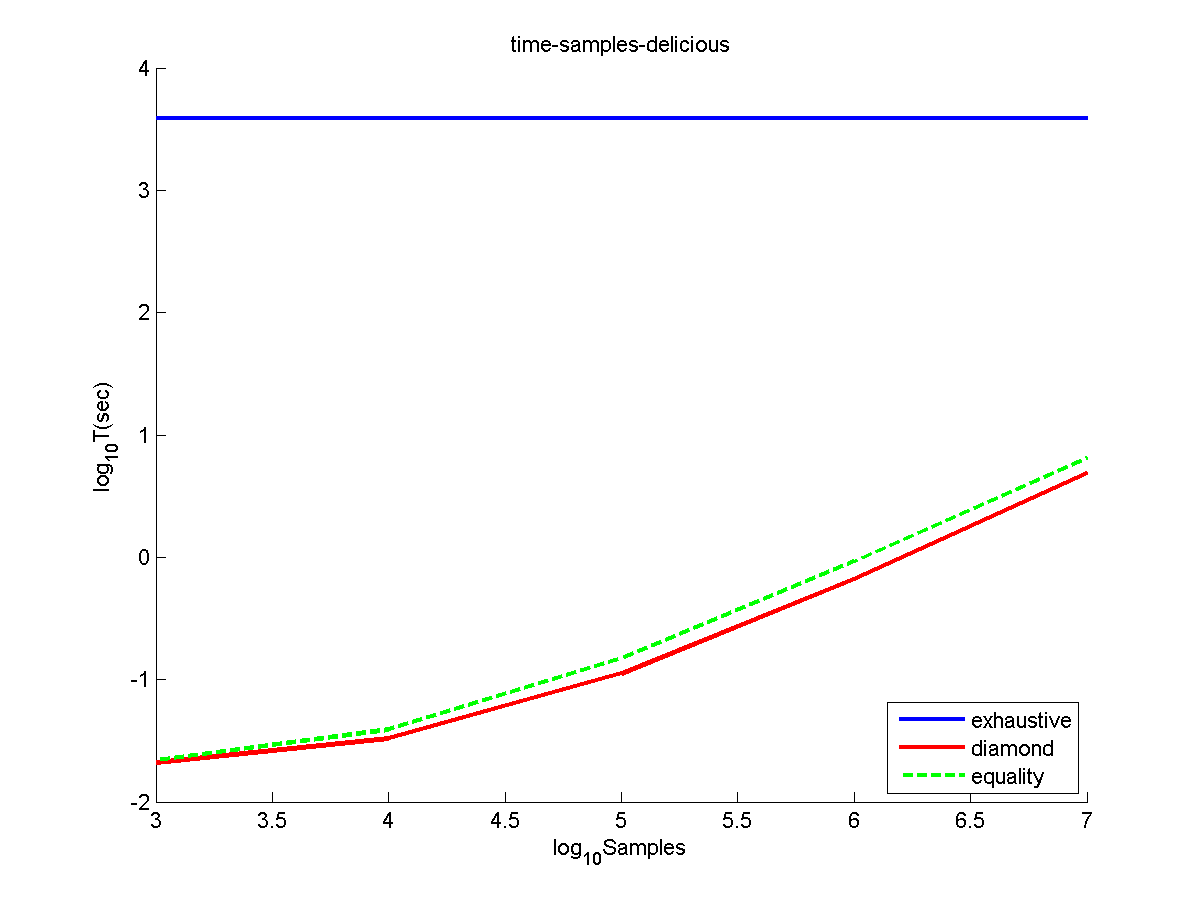
\includegraphics{./img/full/time/time-samples-delicious}
  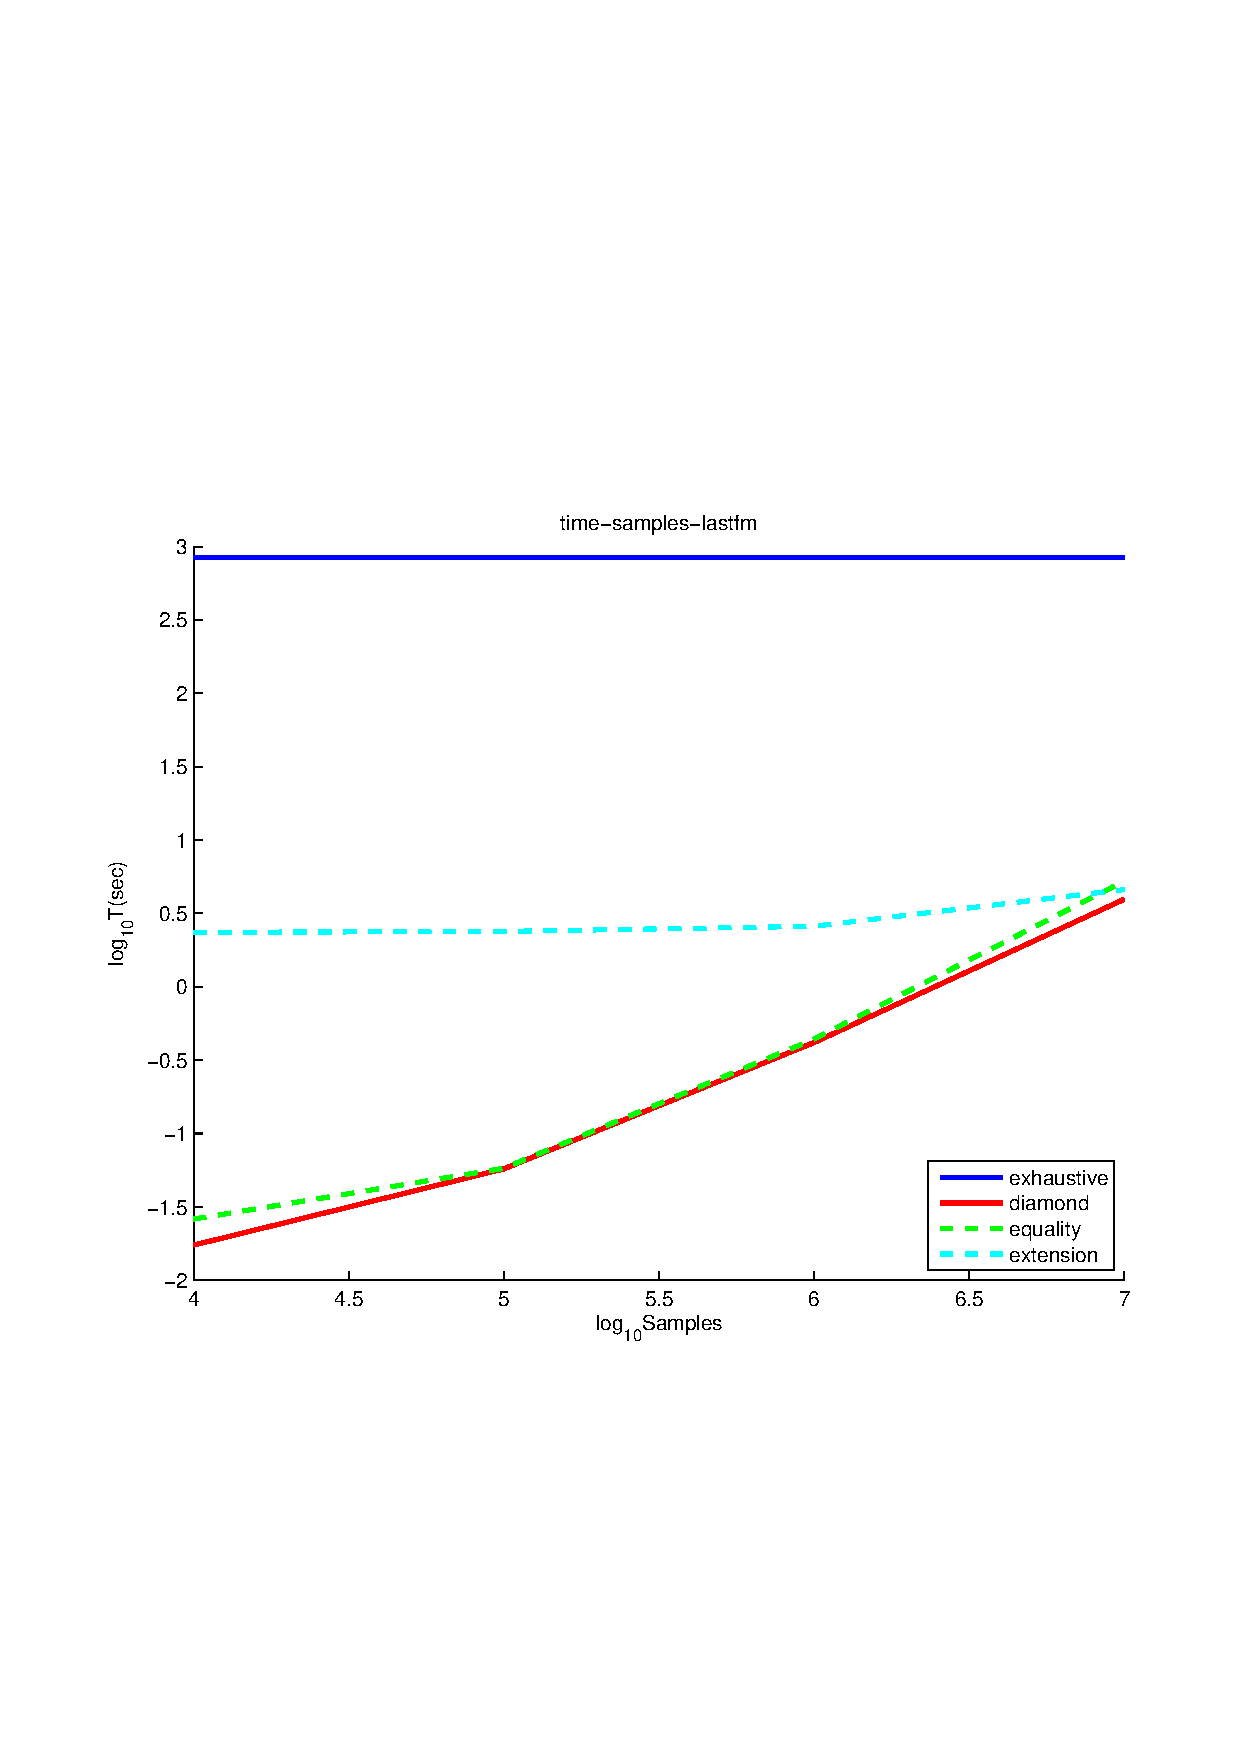
\includegraphics{./img/full/time/time-samples-lastfm}
  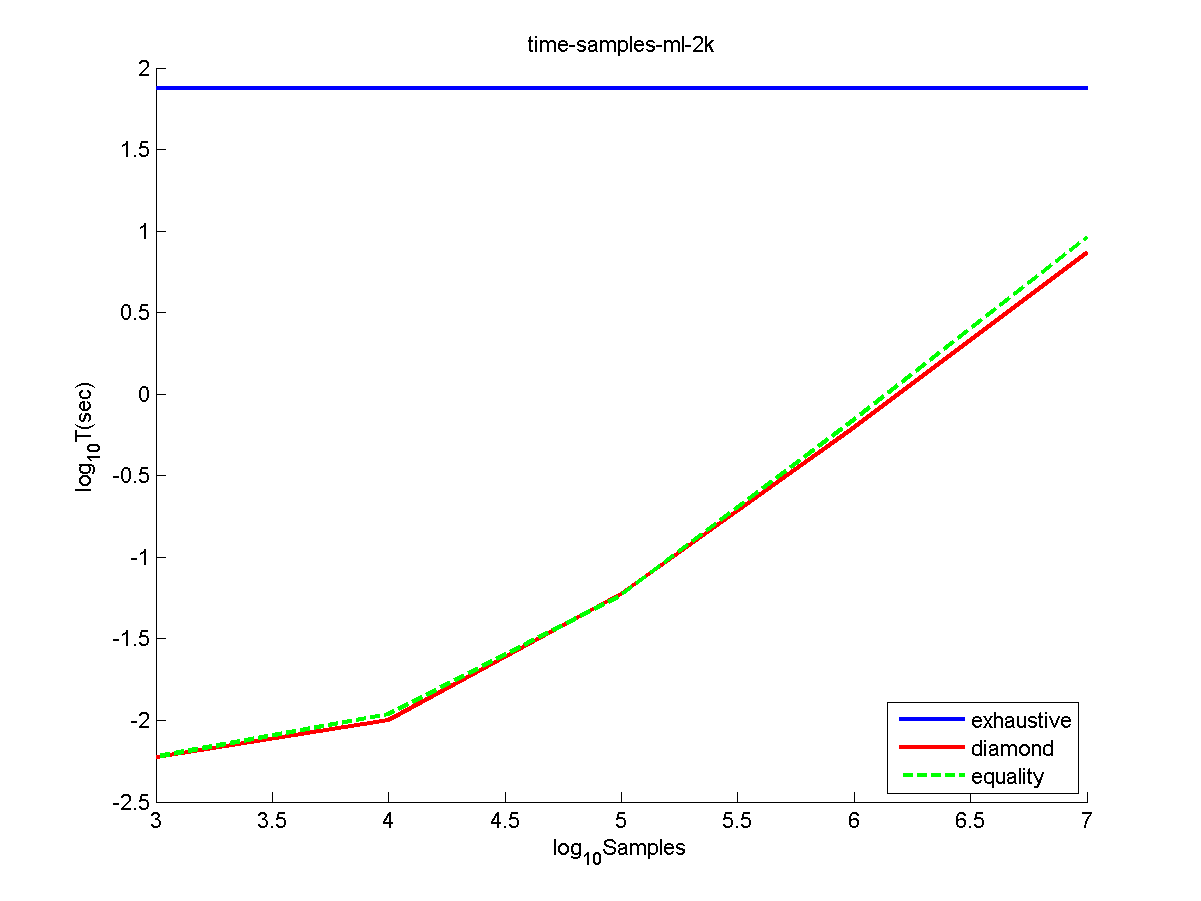
\includegraphics{./img/full/time/time-samples-ml-2k}
  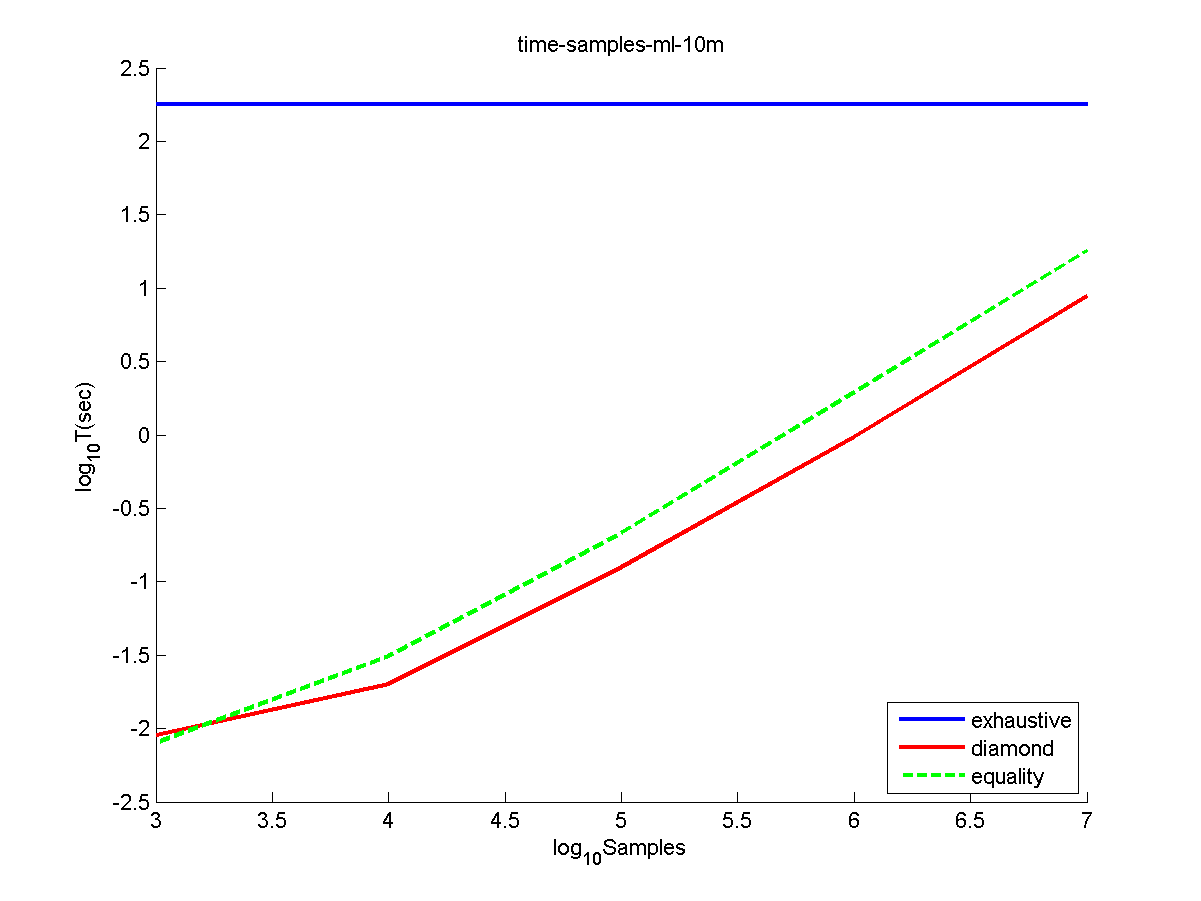
\includegraphics{./img/full/time/time-samples-ml-10m}
  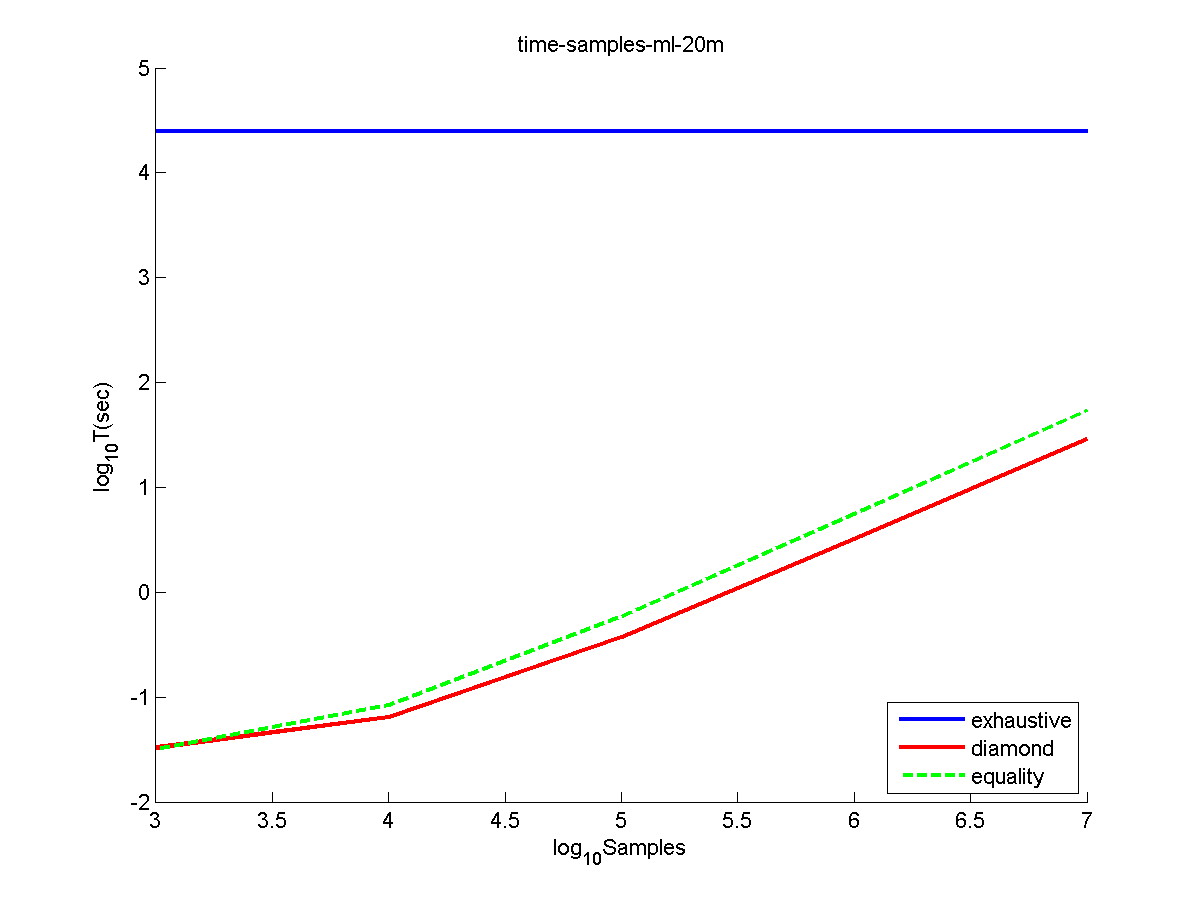
\includegraphics{./img/full/time/time-samples-ml-20m}\\
  \caption{Time for different sampling approaches in different data sets. All methods use the maximum budget that equals to the number of samples}
  \label{fig:Time}
\end{figure}

\subsection{Isotonicity of score}
Given the number of samples, we use different budget to see each method's ability to keep the order.

\begin{figure}[ht]
  \centering
  % Requires \usepackage{graphicx}
  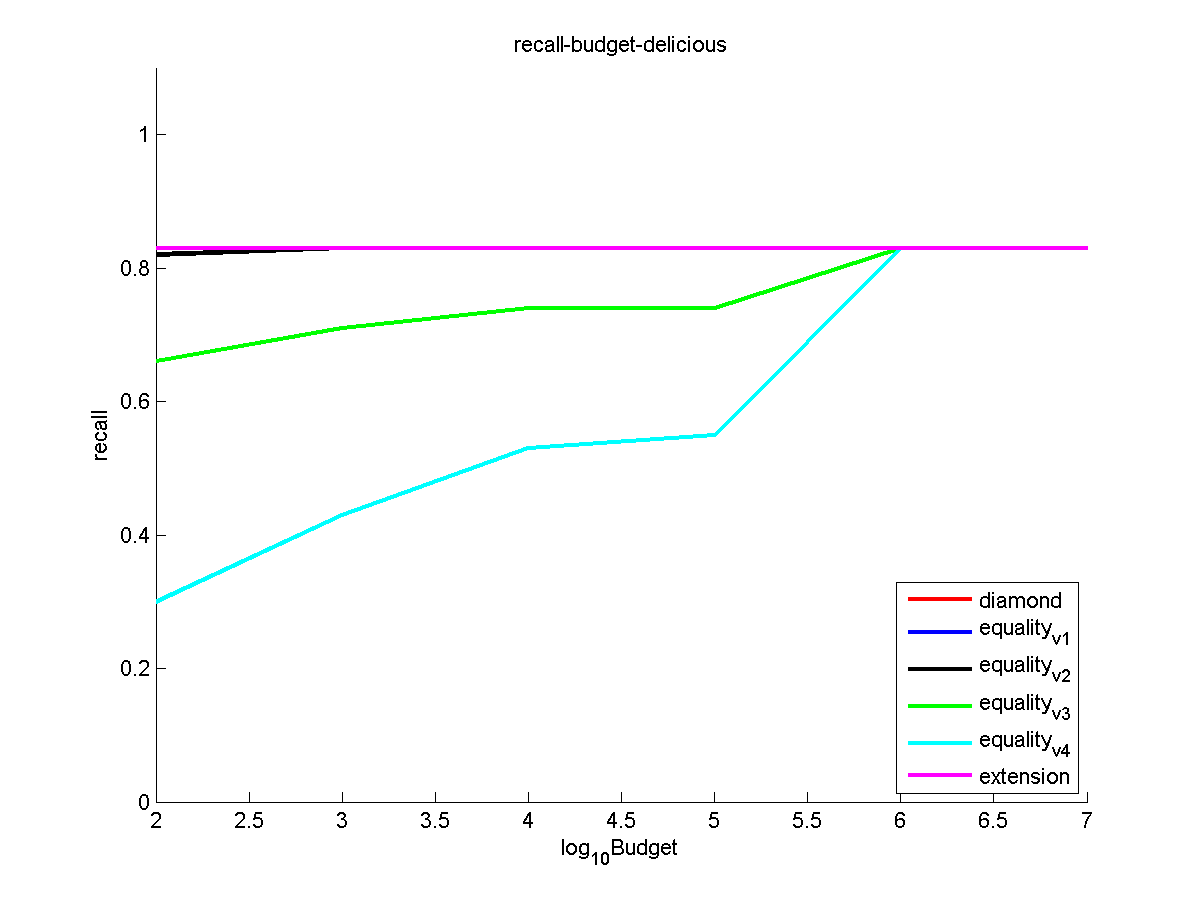
\includegraphics{./img/order/recall-budget-delicious}
  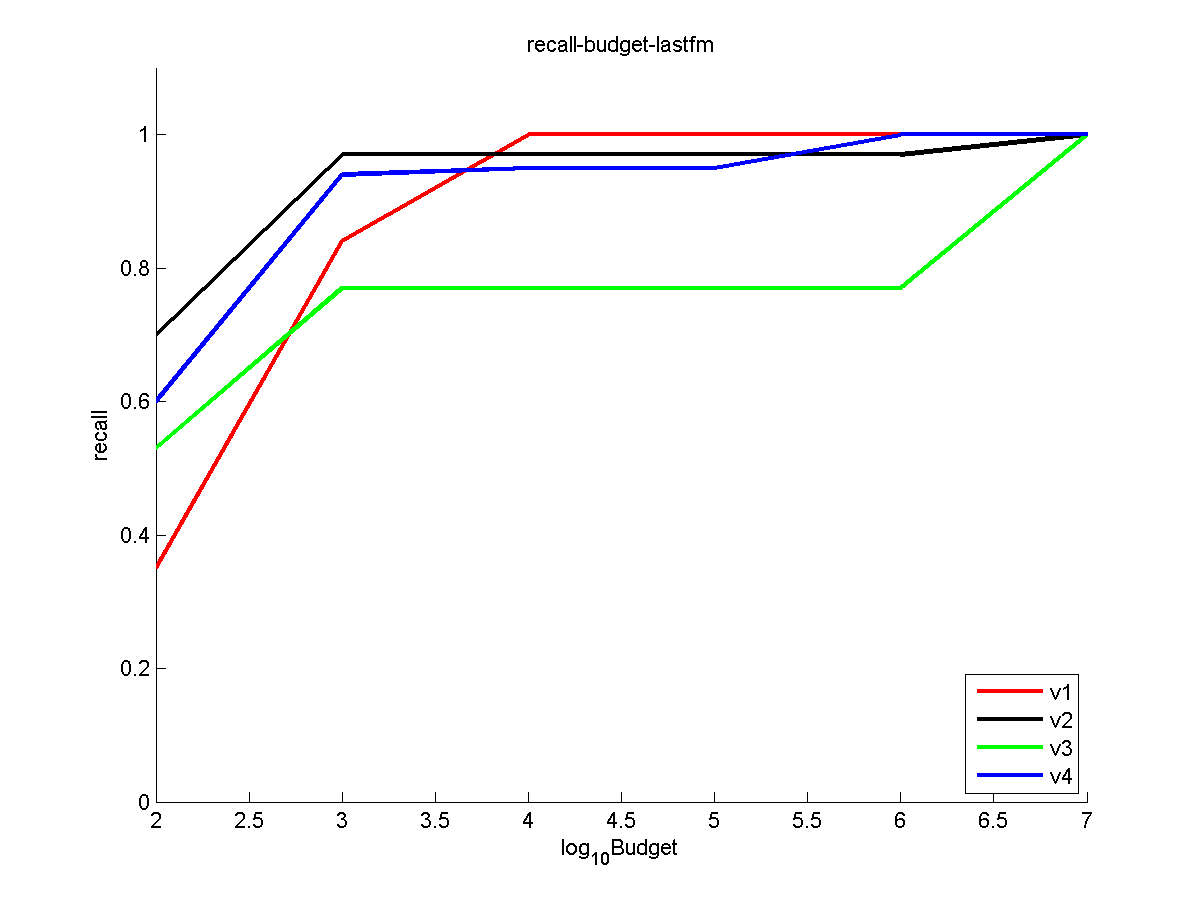
\includegraphics{./img/order/recall-budget-lastfm}
  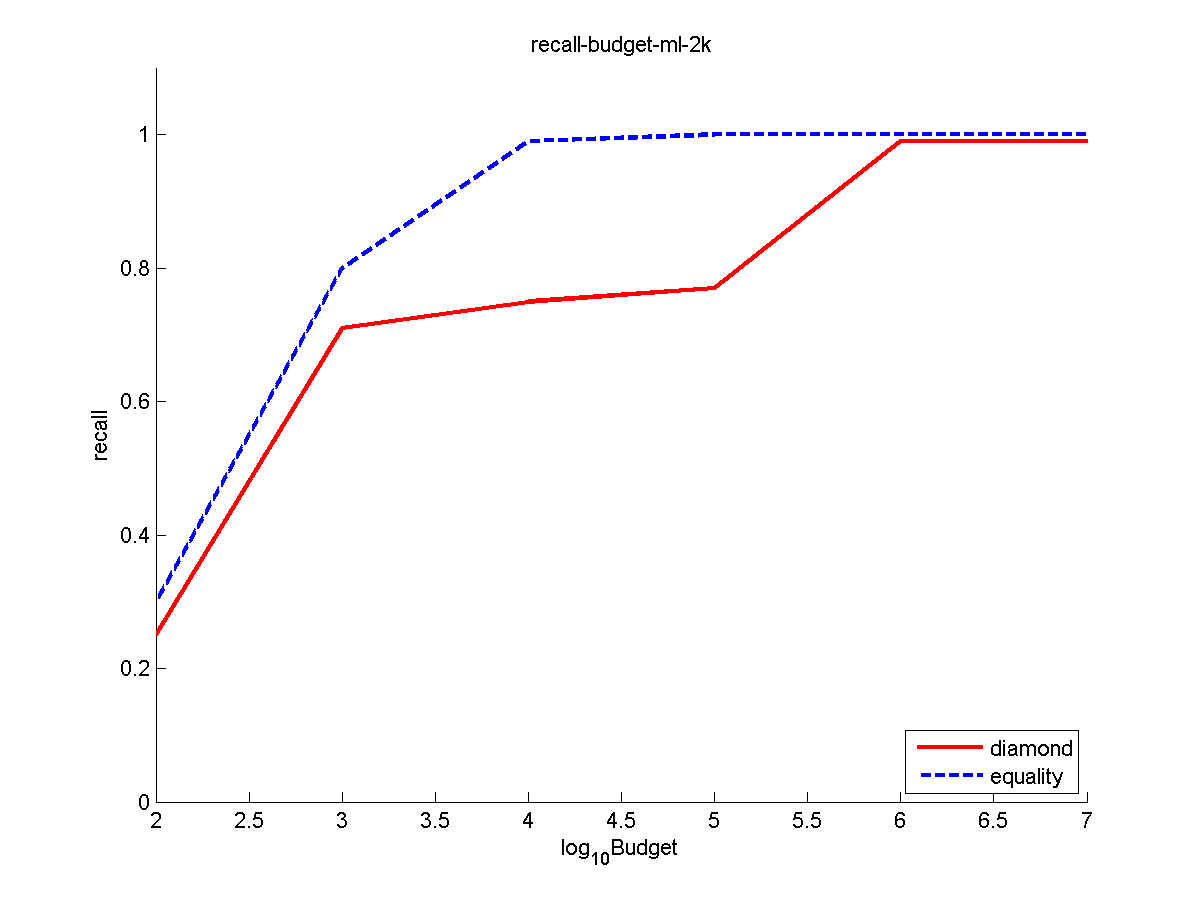
\includegraphics{./img/order/recall-budget-ml-2k}
  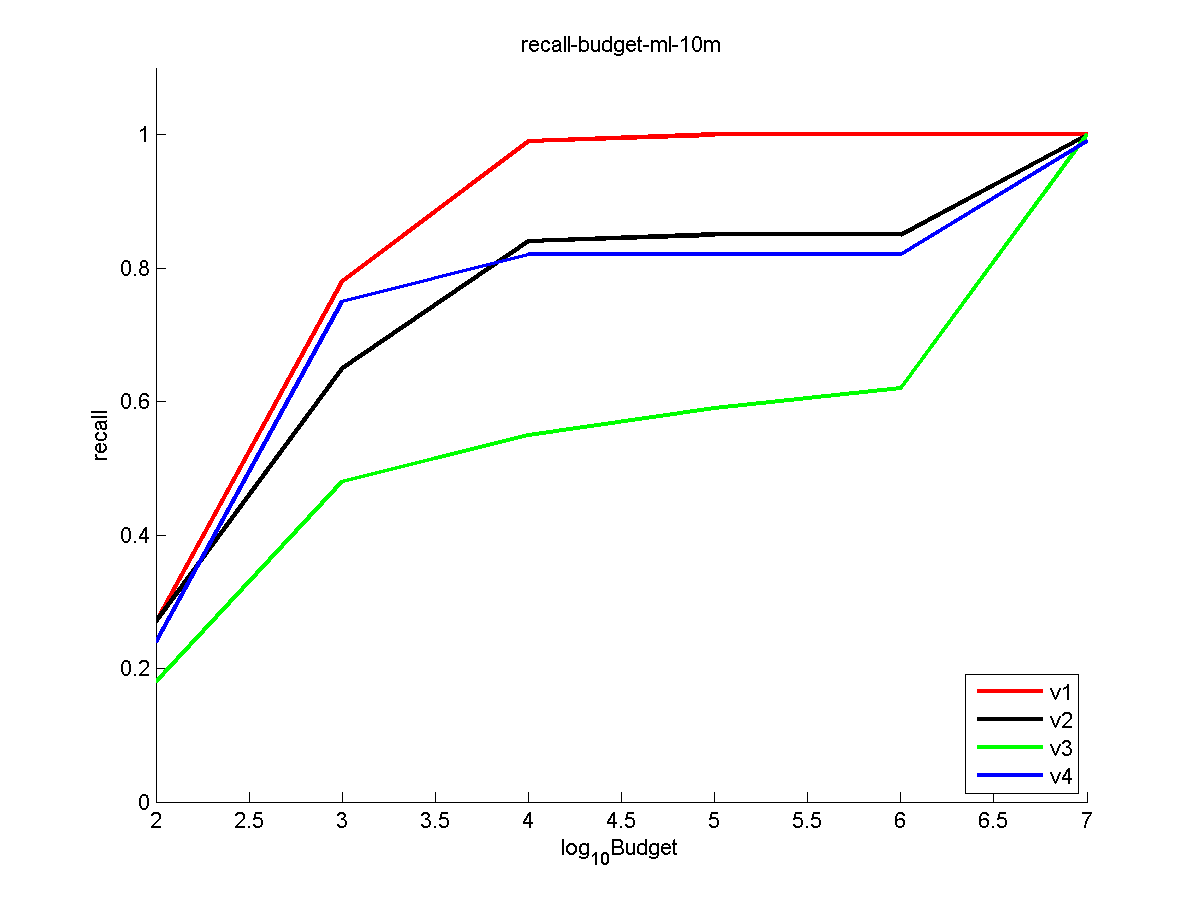
\includegraphics{./img/order/recall-budget-ml-10m}
  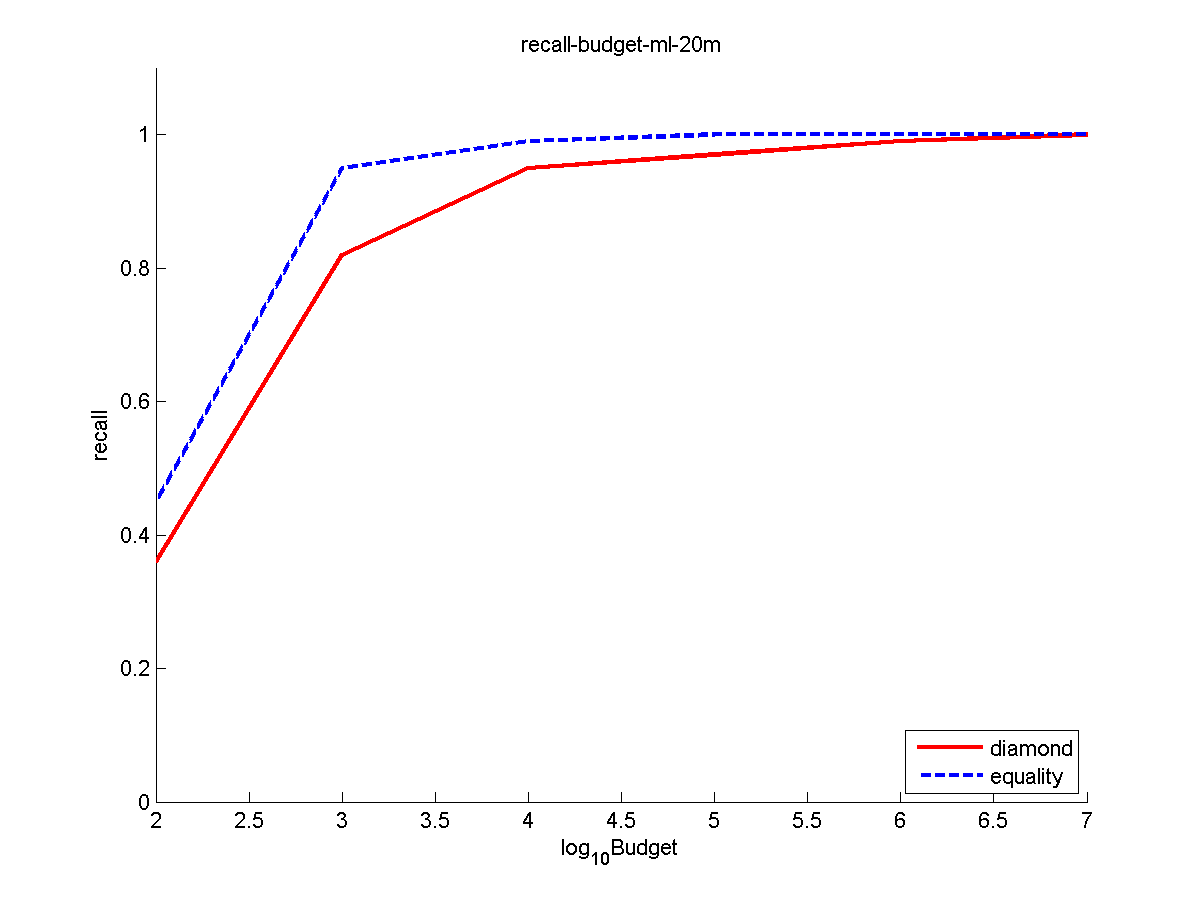
\includegraphics{./img/order/recall-budget-ml-20m}\\
  \caption{Accuracy for different sampling approaches in different data sets. All methods use the same samples $10^6$ and the budget varies form $10^3$ to $10^6$}
  \label{fig:RecallBudget}
\end{figure}
\begin{figure}[ht]
  \centering
  % Requires \usepackage{graphicx}
  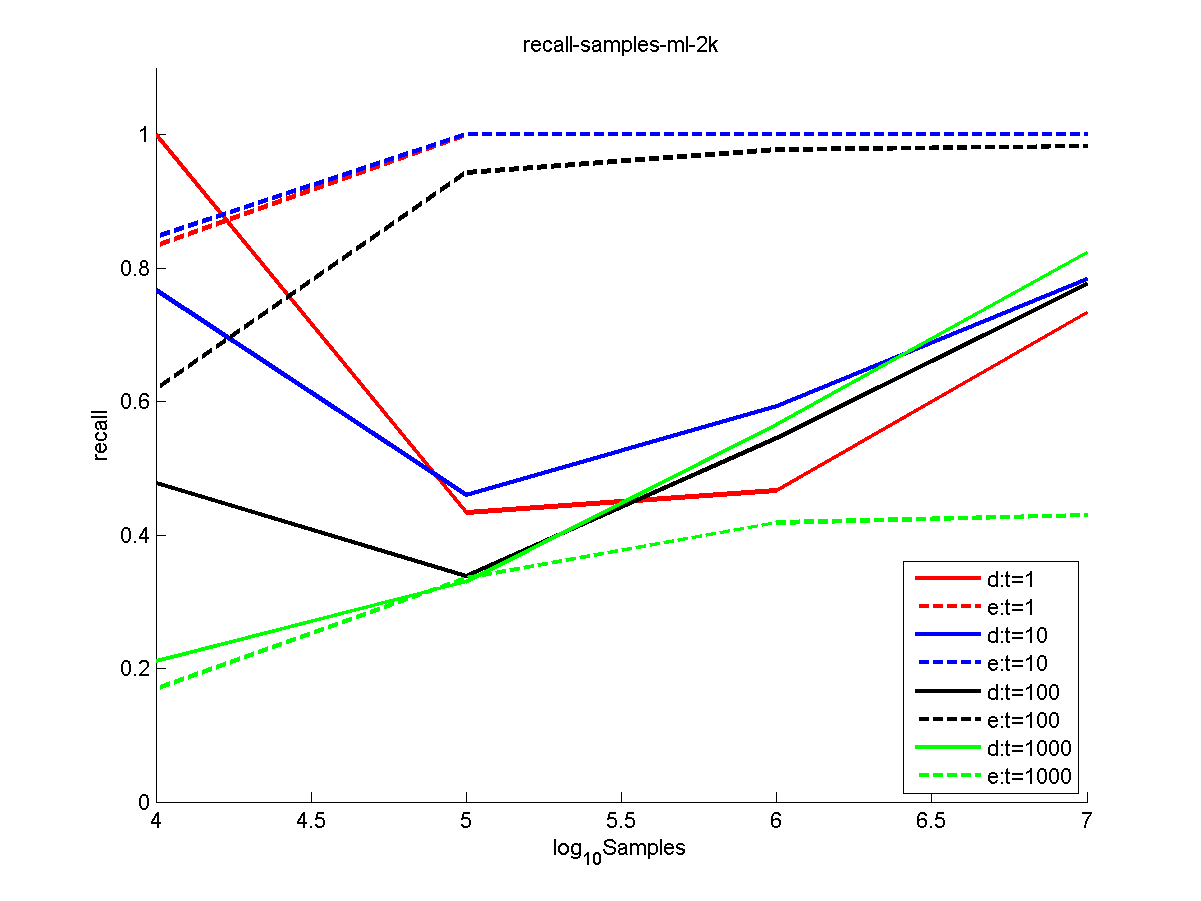
\includegraphics{./img/query/recall/recall-samples-ml-2k}
  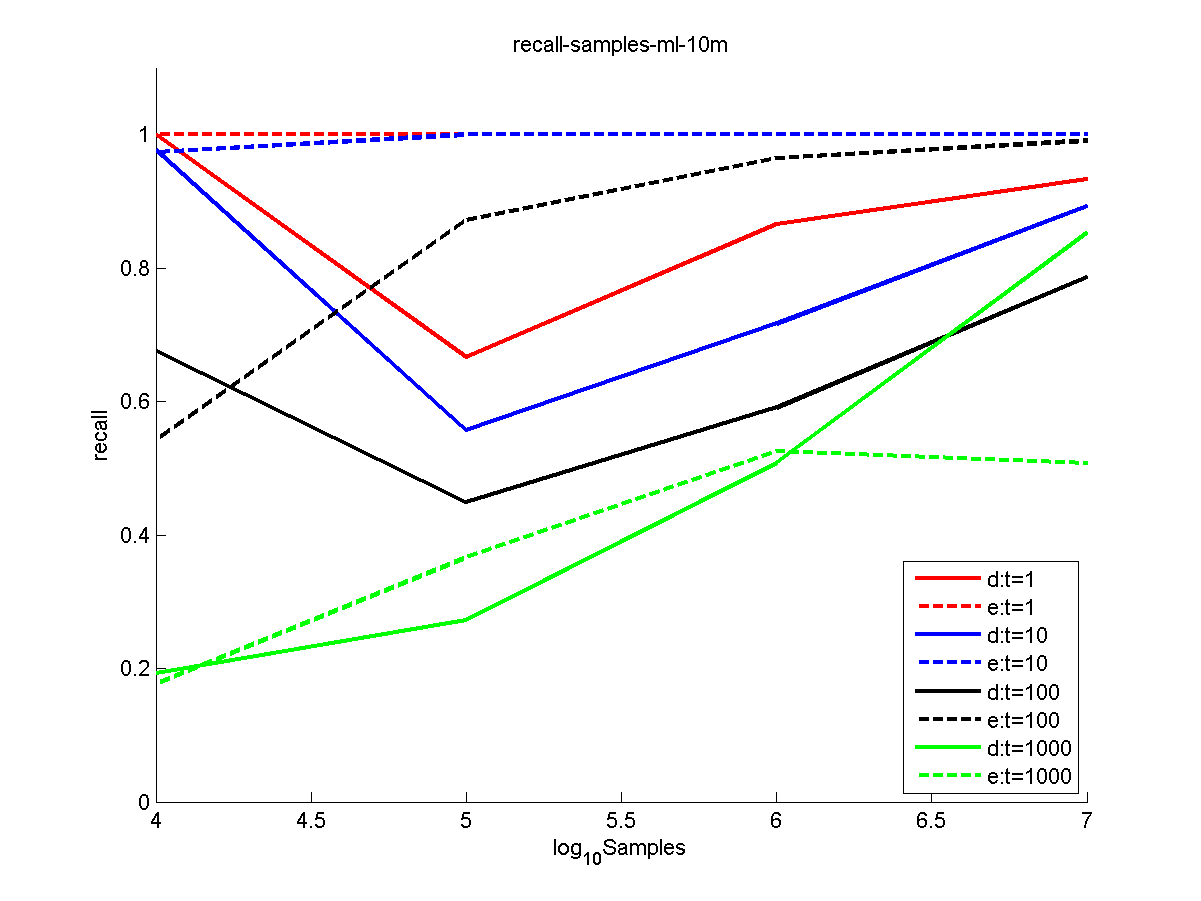
\includegraphics{./img/query/recall/recall-samples-ml-10m}
  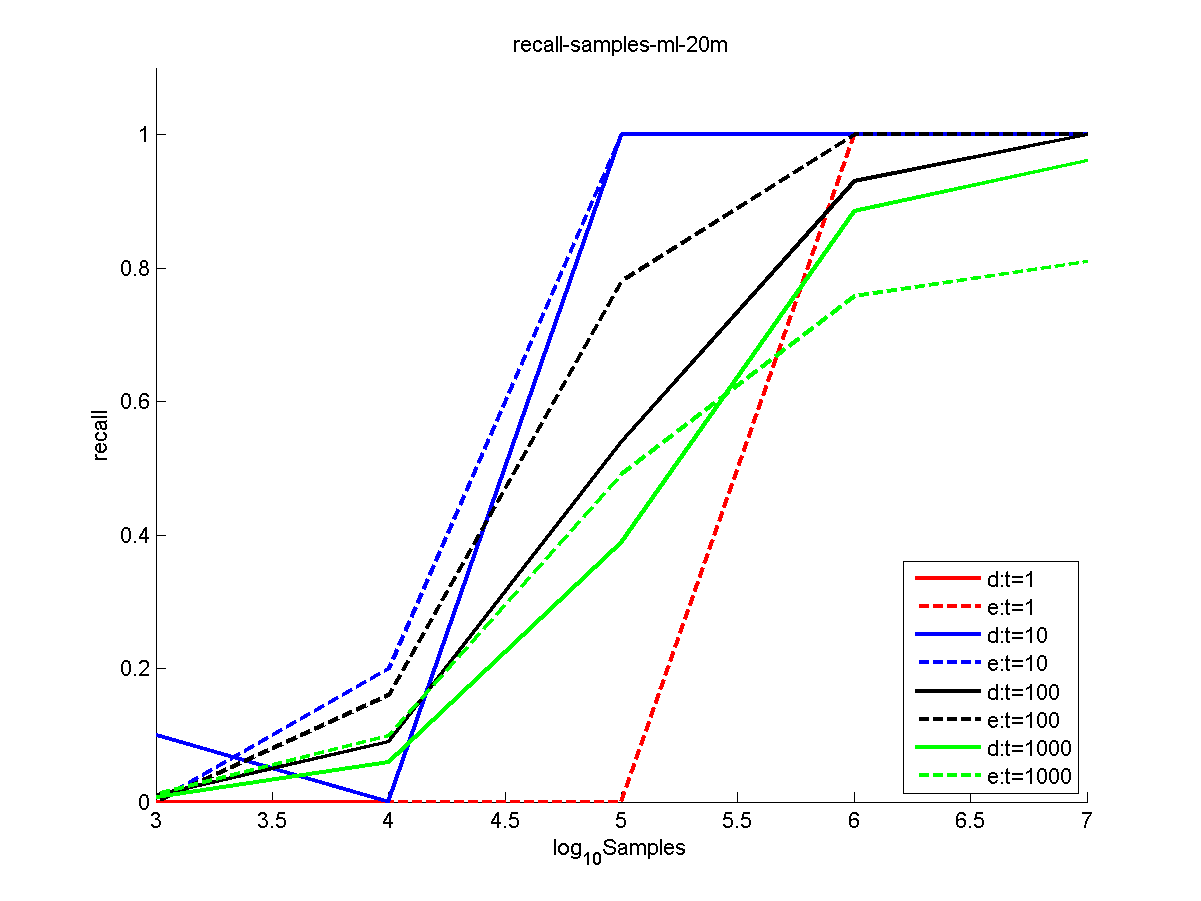
\includegraphics{./img/query/recall/recall-samples-ml-20m}\\
  \caption{Accuracy for different sampling approaches in different data sets. All methods use the same samples $10^6$ and the budget varies form $10^3$ to $10^6$}
  \label{fig:RecallBudget}
\end{figure}

\subsection{Sampling for Queries}
We use the list of sub-path to save the computation of sampling for queries, and we will show the recall when we use the sub-indexes pool and not.

\subsection{Other Ranking Functions}





\bibliographystyle{aaai}
\bibliography{IIP}
\end{document}
